\documentclass[a4paper, 11pt]{report}

\usepackage{taltech_bsc}

\addbibresource{bibliography.bib}

\begin{document}
\begin{titlepage}
    
\includegraphics{taltech_logo.jpg}

    \begin{center}
        \vspace{35mm}
        \begin{LARGE}
            Flux balance analysis of continuous cultivation for investigating
            the lipogenesis metabolism in \textit{Rhodotorula toruloides}
        \end{LARGE} \\
             Bachelor thesis

        \vspace{30mm}
        \hfill
        \parbox{50mm}{
            Student: Maive Hanni \\
            Supervisor: Alina Rekena, Department of Chemistry and Biotechnology, Early Stage Researcher \\
            Study program: Applied Chemistry and Gene Technology
            }

        \vfill
        Tallinn 2024
    \end{center}
\end{titlepage}

\begin{titlepage}
    
\includegraphics{logo.jpg}

    \begin{center}
        \vspace{35mm}
        \begin{LARGE}
            \textit{Rhodotorula toruloides} lipogeneesi uurimine, kasutades metaboolsete voogude analüüsi
        \end{LARGE} \\
            Bakaluareusetöö

        \vspace{30mm}
        \hfill
        \parbox{50mm}{
            Üliõpilane: Maive Hanni \\
            Juhendaja: Alina Rekena, Keemia ja biotehnoloogia instituut, Doktorant-nooremteadur \\
            Õppekava: Rakenduskeemia ja geenitehnoloogia
            }

        \vfill
        Tallinn 2024
    \end{center}
\end{titlepage}

\chapter*{Declaration}
\thispagestyle{empty}

Hereby I declare that I have compiled the paper independently and all works, important standpoints and data by other authors have been properly referenced and the same paper has not been previously been presented for grading.

Author: Maive Hanni \\
Signature, date


\vspace{2cm}

The paper conforms to requirements in force. \newline
Supervisor: name \\
Signature, date

\vspace{5cm}

Permitted to the defence. 
Chairman of the Defence Committee: Name \\
Signature, date



\tableofcontents

\pagenumbering{arabic} % alusta nummerdust siit
\setcounter{page}{4}

\chapter*{Abstract}
\phantomsection
\addcontentsline{toc}{chapter}{Abstract}

% Kokkuvõte hõlmab töö olulisemad tulemused ja järeldused, töö eesmärgi täidetuse analüüs,
% ettepanekuid töö edasiarendamiseks ning edasiseks uurimistööks antud valdkonnas, maht kuni 1 lk.
% Kokkuvõte ei tohi sisaldada põhiosas käsitlemata seisukohti ja lahendusi.

% Annotatsioon annab lugejale ülevaate töö eesmärkidest, olulisematest käsitletud probleemidest ning
% tähtsamatest tulemustest ja järeldustest. Annotatsioon on töö lühitutvustus, mis ei selgita ega
% põhjenda, kuid kajastab piisavalt töö sisu. Annotatsioon esitatakse mahuga pool kuni üks A4 lehekülge
% lõputöö keeles, millele lisatakse eestikeelse töö puhul inglise keelne Abstract. Võõrkeelse töö puhul
% lisatakse eestikeelne annotatsioon (va ingliskeelse tasemeõppekava lõputöö korral). Erinevates keeltes
% annotatsioonid vormistatakse erinevatele lehekülgedele – annotatsiooni pealkiri on esimese taseme
% pealkiri, mis algab uuest leheküljest.

% A thesis must have an abstract or summary in both Estonian and English. An abstract provides the reader an overview of the objectives of the thesis, the key issues discussed and the most important findings and conclusions. An abstract is a brief introduction, which provides no explanations or arguments but reflects adequately the content of the thesis. An abstract must be half to one A4 page long. An abstract must not contain statements not discussed in the body text. Abstracts in different languages shall be written on separate pages. The version in the language of the thesis should come first.

The transition towards bioeconomy to reduce the dependence on fossil-based resources, necessitates innovative methods for producing chemicals and fuels from sustainable materials. The current production of biodiesel from oilseeds and waste oils is insufficient to meet the global demand of the biodiesel industry, highlighting the need for second-generation oleochemicals derived from non-edible sources. Microbial oils (SCOs), which utilize low-value waste streams and do not compete with the food sector, are a promising source of fatty acids for oleochemical production.
The non-conventional, oleaginous yeast \textit{Rhodotorula toruloides} is one of the most promising yeasts for bioproduction of oleochemicals.
Although its metabolic pathways that enable lipid production are defined, the way of enabling such a high lipid production is not fully understood.

Genome-scale metabolic models (GEMs) can be used to predict metabolic fluxes, enabling a greater understanding of cellular physiology, providing valuable information for metabolic engineering to develop better microbial factories. Several genome-scale metabolic models have been developed for \textit{Rhodotorula toruloides}, but a comprehensive overview of simulations focused on central carbon metabolism with these models has not yet been presented.
The objective of this thesis was to compare the predictions of central carbon metabolism focused on lipogenesis of four classical GEMs of \textit{R. toruloides} (rhto-GEM, iRhtoC, Rt\_IFO0880, and Rt\_IFO0880\_LEBp2023) using FBA optimized for biomass maximization and NGAM minimization over five increasing specific growth rates. The simulations showed that over the growth rates, investigated fluxes increased linearly. 

In regard to cofactor NADPH metabolism, the rhto-GEM and iRhtoC models predicted most of the NADPH to be produced through oxPPP, while the Rt\_IFO0880-based models predicted that most of the NADPH is produced by alcohol dehydrogenase, aldehyde dehydrogenase, or homoserine dehydrogenase, depending on the objective function and specific growth rate, indicating the need for a consensus genome-scale metabolic model of \textit{R. toruloides}.




\chapter*{Annotatsioon}
\phantomsection
\addcontentsline{toc}{chapter}{Annotatsioon}

\chapter*{Abbreviations}
\phantomsection
\addcontentsline{toc}{chapter}{Abbreviations}

% Lühendite loetelus esitatakse lühendid tähestikulises järjekorras. Lühendite ning mõistete sõnastikku
% lisatakse töö põhitekstis kasutatud uued ning ka mitmetähenduslikud üldtuntud terminid. Olenemata
% lühendi lisamisest tabelisse, tuleb see töö põhiosa tekstis esmakordsel mainimisel alati lahti seletada.
% Vajadusel võib lühendite seletused esitada ka põhitekstis nende esmamainimisel.

% Tahestiku jrkr
\begin{acronym}
\acro{ACL}{ATP-citrate lyase}
\acro{acetyl-CoA}{acetyl-coenzyme A}
\acro{ATP}{adenosine triphosphate}
\acro{BiGG knowledge-base}{biochemical, genetic, and genomic knowledge-base}
\acro{C/N}{carbon-to-nitrogen ratio}
\acro{cMDH}{cytosolic malate dehydrogenase}
\acro{DNA}{deoxyribonucleic acid}
\acro{DW}{dry cellular weight}
\acro{FAME}{fatty acid methyl ester}
\acro{FAEE}{fatty acid ethyl ester}
\acro{FBA}{flux balance analysis}
\acro{GAM reaction}{growth-associated maintenance reaction}
\acro{GEM}{genome-scale model}
\acro{ME}{malic enzyme}
\acro{NADPH}{nicotinamide adenine dinucleotide phosphate (reduced form)}
\acro{NGAM reaction}{non-growth-associated maintenance reaction}
\acro{PPP}{pentose phosphate pathway}
\acro{RNA}{ribonucleic acid}
\acro{SBML}{Systems Biology Markup Language}
\acro{SCO}{single-cell oil}
\acro{TAG}{triacylglycerol}
\acro{TCA cycle}{tricarboxylic acid cycle (citric acid cycle)}
\end{acronym}


\chapter*{Introduction}
\phantomsection
\addcontentsline{toc}{chapter}{Introduction}

% Sissejuhatuses esitatakse lühidalt (1-2 lk) probleemi tutvustus ja teema valiku põhjendus, töö probleem
% ja eesmärk. Tuuakse välja teema aktuaalsus ja uudsus.

% Introduction is going to be still about how FBA in R. toruloides has been analyzed on a rather general level, but to aid metabolic 
% engineering, we need to understand it more. Then you introduce different models, describe what 
% they did, mention that in S. cerevisiae very detailed FBA studies have been carried out, so more 
% specific FBA analysis in R. toruloides is necessary… That is why most of the writing is good to 
% do at the end when all is more clear.

 %alates siit kuni lisadeni laheb sisukorda

%%%%%%%%%%%%%%%%%%%%%%%%%%%%%%%%%%%%%%%%%%%%%%%%%%%%%%%%%%%%%%%%
             %Töö sisuline osa
%%%%%%%%%%%%%%%%%%%%%%%%%%%%%%%%%%%%%%%%%%%%%%%%%%%%%%%%%%%%%%%%

\chapter{Theoretical background}

\section{Need for new technologies to reduce reliance on fossil-based resources} 
% Lisaksin teoreetilise osa esimeseks peatükiks üldise kirjelduse vajadusest vähendada fossiilsete materjalide osakaalu ning selle mitigeerimiseks 
% on ühe võimalusena võimalik kasutada biotehnoloogilisi protsesse, mis suudavad konverteerida jääk-biomassi erinevateks kemikaalideks ning materjalideks. 
% Siit saaks siis otse edasi liikuda R. toroloidese kirjeldusele, kui ühele potentsiaalsele rakuvabrikule biotehnoloogiliste protsesside läbiviimisel. % Petri soovitus

% Due to the massive increase in the utilization of petroleum, it has 
% been predicted that the world will run short of petroleum by the year 
% 2070 \cite{ShieldsMenard2018}. 

% Besides, its widespread usage has also brought global warming 
% and health concerns due to the release of greenhouse and toxic gases 
% such as carbon monoxide, carbon dioxide, methane, and chlorofluorocarbons. Therefore, alternative energy sources that are easily accessible, 
% greener, and readily available are highly required. Due to properties 
% such as non-toxic, biodegradability, being sulfur-free, and the ability of 
% production from renewable sources, biofuels have gained the interest as 
% an alternative to petroleum. \cite{Saini2020}

Many countries globally are developing a bio-based economy to fight climate change and to lower the
reliance on fossil-based resources \cite{Zuiderveen2023}. In Europe, 
the Bio-Economy Strategy was developed to steer Europe towards a sustainable 
bio-based economy and it was reinforced in the European Green Deal aiming for 
climate neutrality by 2050 \cite{Research2018}. Bio-based products may enhance environmental 
sustainability compared to fossil based equivalents \cite{Zuiderveen2023}.

The shift towards a bioeconomy needs novel processes for production of chemicals, materials, 
and liquid fuels from sustainable substrates, that offer improved life cycle 
assessments, and use less energy to produce. Advancements have highlighted the 
potential of chemicals derived from plant oils and animal fats as alternative 
feedstocks to the petrochemical industry. \cite{Lopes2020} 
Biodiesel is synthesized through the 
transesterification of triacylglycerols with short-chain alcohols 
(primarily methanol or ethanol) to yield monoalkyl esters, specifically fatty acid methyl esters (FAMEs) 
and fatty acid ethyl esters (FAEEs) \cite{Koutinas2014}.

% These bioproducts comprise a broad spectrum of molecules that can be utilized in 
% various applications such as biofuels, cosmetics, plastics, 
% surface coatings, surfactants, lubricants, paints, etc. \cite{Lopes2020}. Bad citation

The demand for vegetable oils has increased rapidly due to the expansion
of the demand for edible oils in the food market (representing over 80\%).
The increasing demand in biodiesel sector also represents an increasing part in the growth of the demand of vegetable oils. \cite{rosillo2009global}
But the production of biodiesel from oilseeds and waste oils does not sustain the 
global demand \cite{Koutinas2014} and the recent food crisis has shown the 
need for the development of second-generation biofuels derived from non-edible sources, 
such as lignocellulosic raw materials and industrial waste streams \cite{Koutinas2011}.

Another promising source of fatty acids for oleochemical production are microbial oils, also called single-cell oils (SCOs), that represent
the triacylglycerides produced by microorganisms \cite{Bonturi2017}.
Research has focused on the development 
of biodiesel production from SCO that are produced via fermentation using oleaginous microorganisms (microorganisms 
capable of accumulating lipids at more than 20\% of the total cellular dry weight (DW)). 
Biodiesel production from SCO relies on the utilization of low-value waste streams 
or residues, thus presenting a sustainable alternative for biofuel production. 
Moreover, the production of SCOs does not require land or other resources that are typically used for food production 
and it is not influenced by season or climate. \cite{Koutinas2014} 


\section{\textit{Rhodotorula toruloides}} % {Physiological characteristics} % General Physiological characteristics {Central carbon metabolism}

\textit{Rhodotorula toruloides} (previously \textit{Rhodosporidium toruloides}) is an oleaginous yeast
which can accumulate lipids up to 76.1\% of cell dry weight \cite{Li2007}. 
What is more, \textit{R. toruloides} has good tolerance to inhibitory compounds that are naturally found in biomass hydrolysates \cite{Hu2009}.
\textit{Rhodotorula toruloides} is an exceptional microbial lipid producer and has recently emerged as one of the most promising yeasts for bioproduction \cite{Wu2023, Park2018}.

\textit{R. toruloides} occurs naturally in leaves, soil, sea water, etc. It has a broad substrate range, 
which has made this yeast a popular for producing biological oils from inedible 
substrates such as pentose sugars and crude glycerol. 
The majority of the lipids produced by \textit{Rhodotorula toruloides} are
triacylglycerol (TAG) contained long-chain fatty acids (C16:0 
(palmitic acid), C16:1 (palmitoleic acid), C18:0 (stearic acid), C18:1(oleic acid), and C18:2 (linoleic acid)) and they
are comparable to vegetable oils \cite{Li2007, Vasconcelos2019}.
\textit{R. toruloides} lipid fraction contains also carotenoid pigments, 
omega-3 linolenic acid and heptadecenoic acid,
which makes it a promising organism for production of pharma- and nutraceuticals \cite{Buzzini2007}. 

Fatty acids mainly accumulate as TAGs, and they are
produced via four enzymatic reactions that require 1 adenosine triphosphate (ATP) and 2 nicotinamide adenine dinucleotide phosphate (NADPH) molecules for adding 1 acetyl-coenzyme A 
(acetyl-CoA) to the fatty acid chain \cite{Lian2015}. In fatty acid synthesis and elongation, Acetyl-CoA is the donor of C2-carbon.
NADPH is required for reduction steps and it is mainly produced by malic enzyme (decarboxylating malate dehydrogenase, ME), 
and by glucose 6-phosphate dehydrogenase and phosphogluconate dehydrogenase in the pentose phosphate pathway (PPP). \cite{Tehlivets2007}

Metabolic pathways producing acetyl-CoA and a cofactor NADPH have been the main focus of metabolic studies in \textit{R. toruloides}. Compared to \textit{Saccharomyces cerevisiae}, \textit{R. toruloides} has several different enzymatic pathways that facilitate the generation of lipid precursors. Important difference is that \textit{R. toruloides} possesses the enzyme ATP-citrate lyase (ACL). ACL has been demonstrated to be upregulated in \textit{R. toruloides} during lipid accumulation \cite{Zhu2012} and it has been suggested to be the main source of acetyl-CoA for lipid synthesis in oleaginous species \cite{Vorapreeda2012}.

Proteomics analysis of \textit{R. toruloides} has suggested that NADPH is mainly produced through the pentose phosphate pathway (when grown on xylose and glucose) but the role of malic enzyme is not clearly understood. The role of phosphoketolase in the generation of acetyl-CoA has not been acknowledged previously \cite{Zhu2012}. Lipid biosynthetic reactions downstream of acetyl-CoA synthesis do not differ between oleaginous and non-oleaginous yeast species \cite{Tiukova2019}.


\section{Overview of growth laws in oleaginous microorganisms}

It has been well-established that an imbalance of nutrients in the culture medium 
triggers lipid accumulation in oleaginous microorganisms. When a crucial nutrient, 
typically nitrogen, is depleted, cells continue to assimilate excess carbon substrate and transform it into storage fat. \cite{Ratledge2002}
Thus, the carbon-to-nitrogen ratio (C/N) is a significant factor in initiating lipid accumulation \cite{Lopes2020}.
The cells take in carbon faster than they can convert it into new cells, so the surplus carbon is stored by turning it into lipid. 
This lipid accumulation necessitates a slower cell growth rate, allowing the excess carbon to be assimilated more quickly 
than it can be converted into biomass, thus directing the surplus carbon into lipid. This process of lipid accumulation 
can also be accomplished in continuous culture with oleaginous yeast, where it is essential to maintain a sufficiently 
low dilution rate (growth rate) to enable the cells to assimilate the glucose. Continuous cultivation 
studies have clearly demonstrated that the lipid synthesis rate is slower than the maximum growth rate. \cite{Ratledge2002}

The first major biochemical distinction identified between oleaginous and non-oleaginous yeast species was the presence 
of ATP-citrate lyase in oleaginous yeast during lipid accumulation. This enzyme has been shown to be crucial 
for a eukaryotic microbial cell to accumulate significant amounts of triacylglycerol lipids. Yeasts without ACL 
invariably had low lipid cell contents. However, some yeasts that had ACL activity but did not accumulate lipids, 
suggesting that some other enzyme activities are also necessary for lipid accumulation. \cite{Ratledge2002}

It has been found that another important enzyme in lipogenesis is malic enzyme, which generates NADPH, that is used by fatty acid synthetase. 
NADPH is also generated by glucose-6-phosphate dehydrogenase, phosphogluconate dehydrogenase, and NADP-dependent 
isocitrate dehydrogenase. When malic enzyme activity was inhibited using selective inhibitors (sesamol), lipid 
content in the cells decreased by almost 90\% (from 24\% of the cell biomass to 2\%), without significantly 
affecting growth. This led to the conclusion that sesamol was specifically inhibiting both the cytoplasmic 
and membrane-bound malic enzymes, and without malic enzyme, the cell was unable to accumulate lipid or carry 
out its desaturations. \cite{Ratledge2002}

Wynn and Ratledge (1997) further demonstrated that in a mutant of \textit{Aspergillus Nidulans} that lacked malic enzyme activity, 
only half the lipid that had been previously produced by a competent strain under nitrogen-limited growth 
conditions, was now produced. Fatty acid biosynthesis itself was still functional, and phospholipids were 
be produced. Meaning that the cells can function without malic enzyme, but they cannot produce 
storage triacylglycerols in any significant quantity - without malic enzyme activity, the flow of carbon from glucose to 
lipid was significantly reduced, and only essential lipids were produced, presumably using other sources of NADPH. \cite{Ratledge2002}



\section{Overview of microbial cultivation methods}

% Here you have to explain that in biotechnology, especially with industrial applications like R. toruloides, microbes are 
% grown in bioreactors from small to large scale. What parameters are controlled in cultivations. Don’t be afraid to cite old books 
% or papers that you can find. Please, explain batch, fed-batch and steady-state cultivations. Steady state is what is being simulated 
% by GEMs. While sometimes, batch growth is assumed to represent a steady state during the time when cells grow exponentially:)

% Also, please check what experiments have been carried out in those publications of R. toruloides that you have cited throughout 
% this work - you will see batch growth, turbidostat, maybe fed-batch. Pay attention to Shen et al. 2013 and 2017 where steady state 
% cultivation was done. They focused on biomass analyses, but don’t have glucose rates. That’s why we use our latest lab data.

Microorganisms play a crucial role in biotechnology, being utilized for the production of a variety of bioproducts. In an industrial setting, 
these microbes are cultivated in large-scale bioreactors to manufacture biopharmaceuticals, dietary supplements, biofuels, or 
other chemical substances. The cultivation process requires careful control of various parameters to ensure optimal growth 
conditions for the microbes. These parameters include temperature, pH, oxygen levels, agitation (stirring), and pressure. It is
vital to regulate these factors to provide a conducive physical and chemical environment for the cells, thereby 
enhancing their productivity. There are three main methods for microbial cultivation: batch, fed-batch and steady-state. \cite{YangSha2019}

In a batch culture, 
no nutrients are added or waste removed. Microorganisms growing in such a closed culture follow a pattern known as the 
growth curve, which, when plotted against time, reveals different phases.
The first phase of the growth curve, the lag phase, represents a small number of cells (known as an inoculum) introduced into a fresh culture medium, 
a nutrient-rich broth that promotes growth. During this phase, the cell count remains unchanged, but the cells increase 
in size and are metabolically active, producing proteins necessary for growth.
The log phase follows next, where the 
cells divide actively, and their count increases exponentially. Cells in the log 
phase exhibit a constant growth rate and uniform metabolic activity, making them ideal for industrial applications and research work.

However, as the cell count rises during the log phase, several factors contribute to a slowdown in the growth rate. 
Accumulation of waste products, gradual depletion of nutrients, and limited oxygen availability due to increased 
consumption all contribute to this slowdown. This leads to a plateau in the total number of live cells, known 
as the stationary phase. In this phase, the number of new cells created by cell division equals the number of 
cells dying, resulting in a relatively stagnant total population of living cells.
As the culture medium becomes saturated with toxic waste and nutrients get exhausted, cell death outpaces cell 
division, leading to an exponential decrease in the cell count. This phase is named the death or decline phase. \cite{2024Microbial}

Fed-batch fermentation is a variation of batch fermentation. Microorganisms are initially grown under batch conditions, after which nutrients 
are incrementally added to the fermenter throughout the remaining fermentation duration. The addition of fresh nutrients typically results in 
significant biomass accumulation during the exponential growth phase. Therefore, fed-batch fermentation 
is particularly useful for bioprocesses aiming for high biomass density or high product yield when the 
desired product is positively correlated with microbial growth. \cite{YangSha2019}

In industrial applications and research work it is beneficial to keep cells in the logarithmic phase of growth.
A steady-state cultivation, also called chemostat, enables the maintainance of a continuous 
culture thanks to the addition and removal of fluids, adjusted 
to keep the culture in the logarithmic phase of growth. \cite{2024Microbial} 
Fresh medium is continuously added to the fermenter, while used medium, toxic metabolites 
and cells are simultaneously harvested. Unlike fed-batch fermentation, the maximum working volume of 
the vessel does not limit the amount of fresh medium or feed solution that can be added to the 
culture during the process. When the addition and removal rates are equal, 
the culture volume remains constant.The cellular growth rate and environmental conditions, like the concentrations 
of metabolites, remain constant. Steady-state cultures can last for days, weeks, or even months, 
significantly reducing downtime and making the process more economically competitive. \cite{YangSha2019}

% A study attempting to establish optimal production conditions, found that the lipid yield of oleaginous yeasts was greatly 
% improved by using the continuous culture mode, indicating that it is superior to 
% the batch culture mode for lipid production. \cite{Ghazani2022}

% And finally, please explain what is substrate uptake rate and product secretion rate and from what data are they calculated. 
% Please ask me, if you need help with this.

% The density of the culture is defined as the number of cells per volume. \cite{2024Microbial}

% Substrate uptake rate is the rate at which a substrate is taken up by cells. 
% It can be measured by observing the change in substrate concentration in the medium.

% Product secretion rate refers to the rate at which a cell or organism produces and secretes a particular product. It is a 
% measure of how quickly a product is formed and released from the cell. This can be determined by measuring the product concentrations. 

% To calculate these rates, you would typically need data on the concentrations of the substrate and product over time. For example, 
% in a batch cultivation process, you might take multiple samples over time to measure the concentrations of substrate and product, 
% as well as dry cell weight. From this data, you can calculate the specific substrate uptake rate and the specific productivity.

% Specific rate represents a normalized rate with respect to the amount of biomass. %copilot


\section{Genome-scale metabolic modeling} %incl. Constraint-based modeling, kinetic modeling, steady-state, limitations, e.g. regulation

Cellular metabolism involves numerous reactions that are part of the conversion of resources into energy and precursors needed for 
biosynthesis. Rates of these reactions are called fluxes and they illustrate metabolic activity.
Flux of a metabolite results from a combined regulation of many biological levels (transcription, translation, 
post-translational modifications and protein-protein interactions). \cite{Nidelet2016} Hence, metabolic fluxes represent cellular phenotype
under certain conditions and therefore analyzing the flux distribution of metabolites is very useful for studying cell metabolism \cite{Nielsen2003}.
It is difficult to measure intracellular fluxes experimentally, but it is possible to predict these fluxes thanks to metabolic models \cite{Nidelet2016}.

When the first full genome sequences were published in the 1990s, in principle it became possible to identify all the gene products involved in 
given organism's biological processes. This, with well studied biochemistry of metabolism, allowed the reconstruction of metabolic networks on a genome-scale
for a target organism. Such reconstructions, containing biochemical, genetic, and genomic (BiGG) knowledge, can be converted into a mathematical format 
allowing the formulation of genome-scale models (GEMs). \cite{Palsson2009}
Thanks to the fact that GEMs account for all known genes, proteins, and biochemical reactions, it is possible to  
conduct systematic analysis of a given organism's metabolism, where typically the objective is to obtain an overview of possible flux
patterns \cite{Kerkhoven2014, Chen2023}. %Genome-scale metabolic models simulate steady state.
It is possible to integrate omics data and experimental metabolic fluxes to GEMs for generating holistic 
view of metabolism in different physiological states. This enables a greater understanding of cellular physiology, providing valuable information 
for metabolic engineering to develop better microbial factories.

The metabolic reconstruction process usually is very labor- and time consuming. For well-studied, medium genome sized bacteria it can take around six months to reconstruct the model. 
The metabolic reconstruction of human metabolism can take up to two years for six people. The reconstruction process is often iterative, for example the reconstruction of metabolic 
network of \textit{Escherichia coli} has been expanded and refined throughout the last 19 years. Despite growing experience and 
knowledge, it is still not possible to completely automatically reconstruct high-quality metabolic networks which can be used as reliable predictive models. \cite{Thiele2010} 
(See appendix \ref{A:GEM_reconstruction_fig} for more detailed reconstruction process.) 

\subsection{Constraint-based modeling}

Genome-scale metabolic models (GEMs) are commonly used to compute metabolic phenotypes. However, these models also depend on a set of constraints due to various factors that limit cellular functions. These constraints fall into four categories: basic physico-chemical constraints, spatial or topological constraints, condition-dependent environmental constraints, and self-imposed or regulatory constraints. \cite{Price2004}

Physico-chemical constraints are fundamental and provide inviolable constraints on cell functions, including the conservation of mass, energy, and momentum. Topobiological constraints arise from the crowding of molecules inside cells, affecting the form and function of biological systems. For instance, bacterial DNA, which is about 1,000 times longer than a cell, must be tightly packed yet easily accessible for transcription. \cite{Price2004}

Environmental constraints, which are time and condition dependent, include factors like nutrient availability, pH, temperature, osmolarity, and the availability of electron acceptors. These constraints are crucial for the quantitative analysis of microorganisms and require defined media and well-documented environmental conditions for integrating data into accurate and predictive quantitative models. Regulatory constraints are self-imposed and subject to evolutionary change, allowing the cell to eliminate suboptimal phenotypic states. These constraints are implemented in various ways, including the amount of gene products made and their activity. \cite{Price2004}

A significant limitation of conventional GEMs is that they do not account for enzyme abundances and kinetics, which limit metabolic fluxes. These models often assume that the uptake rate of the carbon source limits production, which may oversimplify the situation. \cite{Sanchez2017} The synthesis of enzymes is resource- and energy-intensive, and their catalytic capacities are limited by their kinetics. Furthermore, the quantity of enzymes is space-constrained. \cite{Kerkhoven2022}

An increase in the requirement of an enzyme or a pathway would be a trade-off for other functions. Experimental evidence suggests that resource re-allocation could be an effective strategy in response to nutrient and growth shifts, demonstrating the biological significance of proteome constraints. \cite{Chen2023} Incorporating such constraints into a metabolic model can lead to more realistic results by reducing simulated flux distributions to those that are most economic and limiting the phenotypes that the model can simulate. \cite{Kerkhoven2022}

Genome-scale metabolic models are constrained by three factors: (1) the stoichiometry of the network; (2) preset upper and lower limits for specific reactions; and (3) the assumption of a steady state. \cite{Kerkhoven2014} 
Overview of a reconstruction of a GEMs is shown in the figure \ref{GEMs}.
\begin{figure}[H]
    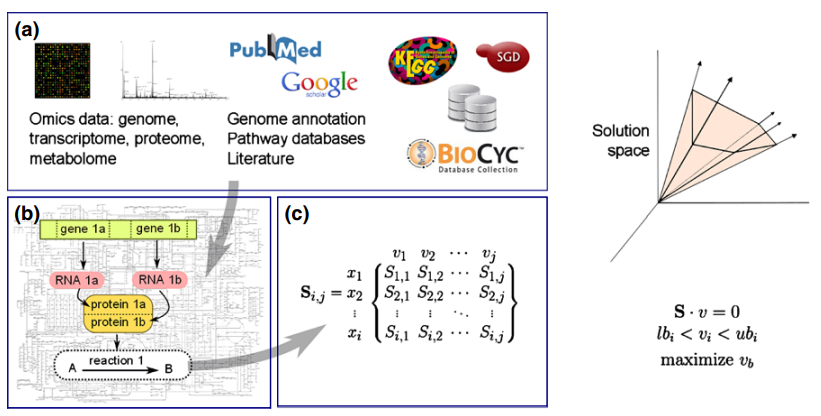
\includegraphics[width=\linewidth]{GEMs.png}
    \caption{Reconstruction of a GEM. (a) The genome annotation is used 
    to reconstruct the draft. (b) Gene-protein-reaction relationships are defined for the metabolic model. 
     (c). A solution space is defined from the constraints applied to the model. Figure is from article \cite{Kerkhoven2014}.}
    \label{GEMs}
\end{figure}

% % Enzyme constrained GEMs - for now these can be excluded

% Integration of enzyme constraints and proteomics data into GEMs was first enabled by the GECKO toolbox \cite{Sanchez2017}, allowing the study of phenotypes constrained by 
% protein limitations. GECKO is a method for enhancement of GEMs with Enzymatic Constraints using 
% Kinetic and Omics data, developed in 2017. This method extends the classical FBA 
% approach by incorporating a detailed description of the enzyme demands for the metabolic reactions in a network, accounting for all types of enzyme-reaction 
% relations, including isoenzymes, promiscuous enzymes and enzymatic complexes. Moreover, GECKO enables direct integration of proteomics abundance data, 
% if available, as constraints for individual protein demands, represented as enzyme usage pseudo-reactions, whilst all the unmeasured enzymes in the network 
% are constrained by a pool of remaining protein mass. \cite{Domenzain2022}

% Every metabolic reaction flux has a
% biological constraint that is equal to the enzyme's concentration multiplied by its turnover number ($k_{cat}$). Enzyme constraint is
% defined as the maximum rate of enzymatic reaction ($v_{max}$) that the metabolic flux cannot exceed. Enzyme-constrained GEMs thereby 
% ensure that each metabolic flux does not exceed its biological maximum capacity, 
% equal to the product of the enzyme's abundance and turnover number. \cite{Sanchez2017}

% Phenomenological constraint is imposed on metabolic flux ($v; mmol/gDCW/h$), formulated as enzyme
% kinetics: $v <=  E \cdot k_{cat}$, where $E$ is protein abundance (mmol/gDCW) and $k_{cat}$ is the enzyme's turnover number (1/s),
% provided with an upper limit on individual or total protein abundances. The integration of
% enzymatic constraints in \textit{S. cerevisiae} has significantly improved phenotype prediction. \cite{Sanchez2017}



\subsection{Flux balance analysis}

% GEMs can simulate metabolic flux distributions by optimization of an objective function that describes the 
% perceived cellular objective that propels 
% metabolism, by flux balance analysis (FBA). \cite{Kerkhoven2022}
Flux balance analysis (FBA) is a mathematical approach for analyzing the flow of metabolites through a metabolic network. It is a commonly employed method for investigating biochemical networks, especially the genome-scale metabolic network reconstructions. FBA enables the computation of flow of metabolites through this metabolic network, thereby making it possible to predict an organism's growth rate or the production rate of a biotechnologically important metabolite. \cite{Orth2010}

The initial phase in FBA involves the mathematical representation of metabolic reactions. The reconstructed genome-scale networks can be transformed into mathematical stoichiometric matrices $\mathbf{S}\in\mathbb{R}^{(m\times n)}$, where each row corresponds to one unique metabolite (for a system with $m$ metabolites) and each column corresponds to an individual reaction ($n$ reactions). \cite{Kerkhoven2014} 
Each column's entries are the stoichiometric coefficients of the metabolites involved in a reaction. A negative coefficient is assigned to each metabolite that is consumed, while a positive coefficient is assigned to each metabolite that is produced. A stoichiometric coefficient of zero is assigned to each metabolite that does not participate in a specific reaction. The stoichiometric matrix $\mathbf{S}$ is sparse, as most biochemical reactions involve only a few different metabolites.
The vector $\mathbf{v}$ represents the fluxes of all the reactions in the network and it has a length of $n$. \cite{Orth2010}

% These stoichiometries impose constraints on the flow of metabolites through the network, defining the solution space of the metabolic network. \cite{Orth2010}

% Other constraints, such as lower and upper bounds for specific reactions, also need to be mathematically described for in silico analysis. Constraints can be classified as either balances or bounds. Balances are associated with conserved quantities and phenomena, such as energy, mass, redox potential and momentum, while bounds limit the numerical ranges of individual variables and parameters (e.g. concentrations, fluxes, kinetic constants). Both types of constraints limit the functional states of reconstructed networks, thereby defining a solution space that represents the phenotypic potential of an organism. \cite{Price2004}


At steady-state (which is simulated by GEMs), there is neither accumulation nor depletion of metabolites in a metabolic network, meaning the rate of production of each metabolite in the network must equal its rate of consumption. This flux balance can be mathematically represented as $\mathbf{S}\cdot \mathbf{v} = \mathbf{0}$. \cite{Price2004}
Any vector $\mathbf{v}$ that satisfies this equation is said to be in the null space of $\mathbf{S}$. In any realistic large-scale metabolic model, there are more reactions than there are compounds ($n > m$). This means that there are more unknown variables than equations, so there is no unique solution to this system of equations. \cite{Orth2010} Thus, the solution space is further constrained by a set of upper and lower bounds on the fluxes ($a_i < v_i < b_i$). 

% Without constraints, the flux distribution may lie at any point in a solution space. When mass balance constraints imposed by the stoichiometric matrix $\mathbf{S}$ and capacity constraints imposed by the lower and upper bounds ($a_i$ and $b_i$) are applied to a network, it defines an allowable solution space. The network may acquire any flux distribution within this space, but points outside this space are denied by the constraints. \cite{Orth2010}

The subsequent step in FBA is to define a biological objective that is relevant to the problem being studied. Even though constraints define a range of solutions, it is still possible to identify and analyze single points within the solution space. For instance, we may be interested in identifying which point corresponds to the maximum growth rate, the rate at which metabolic compounds are converted into biomass constituents (nucleic acids, proteins, and lipids), or to the maximum ATP production of an organism, given its particular set of constraints. FBA is one method for identifying such optimal points within a constrained space. \cite{Orth2010}

Mathematically, the objective is represented by an objective function that indicates how much each reaction contributes to the phenotype. A biomass reaction that drains precursor metabolites from the system at their relative stoichiometries to simulate biomass production is selected by the objective function in order to predict growth rates. This reaction is scaled so that the flux through it is equal to the exponential growth rate $\mu$ of the organism. \cite{Orth2010}

The problem of FBA is to find a vector $\mathbf{v}$ such that it satisfies constraints
\begin{equation*}
    \mathbf{S}\cdot\mathbf{v} = 0, \qquad a_i<v_i<b_i    
\end{equation*}
and maximizes/minimizes the objective function. In order to solve this problem, linear programming methods are used. For example, the COBRA Toolbox \cite{Becker2007} can be used for solving this kind of problems efficiently for large systems of equations. The COBRA Toolbox, freely available in Matlab and Python, uses models saved in the Systems Biology Markup Language (SBML) \cite{Hucka2003} format.
The resulting flux distribution $\mathbf{v}$ maximizes or minimizes the given objective function (see figure \ref{fig:Solution_space}). \cite{Orth2010}
\begin{figure}[H]
    \includegraphics[width=\linewidth]{FBA_solution_space.jpg}
    \caption{Conceptual basis of constraint-based modeling and FBA. The figure is from \cite{Orth2010}.}
    \label{fig:Solution_space}
\end{figure}

% Sampling of the solution space and optimal solution

An alternative approach to FBA involves sampling of the solution space by considering all permissible flux distributions based on mass balance (stoichiometric) and flux capacity constraints. Uniform random sampling of the solution space is a method to understand the permissible metabolic flux space under any environmental condition. The flux distributions derived from this sampling can answer questions about the most probable flux value for any reactions and dependencies between two reactions under given constraints. \cite{Becker2007}

The most commonly used objective function in FBA include maximization of the specific growth rate, ATP generation or a specific product formation \cite{Kerkhoven2014}.
Beyond metabolic costs, additional energetic requirements (in the form of ATP) exist for growth. These requirements account for growth-associated maintenance (GAM) and non-growth-associated maintenance (NGAM). \cite{Feist2007}
GAM accounts for the energy needed for cell replication, including macromolecular synthesis (proteins, deoxyribonucleic acid (DNA), and ribonucleic acid (RNA)). Determining GAM is best achieved through chemostat growth experiments. NGAM represents ATP requirements for cell maintenance that is not related to growth (in GEMs it is noted as an ATP hydrolysis reaction). The rate of this reaction can be estimated from growth experiments. \cite{Thiele2010} These reactions can also be used as objective functions.

FBA is commonly used to assess the biotechnological potential of 
microorganisms and identify genetic modifications that could enhance the cell performance. Its key applications include:
(1) instructions for metabolic engineering;
(2) biological interpretation and discovery through 
contextualizing high-throughput data;
(3) creating a computational framework;
(4) explaining evolutionary aspects;
(5) describing multispecies communities. \cite{Kerkhoven2014}

However, FBA has limitations. It lacks kinetic parameters, preventing the prediction of metabolite concentrations. Additionally, it only works at steady state and does not fully account for regulatory effects, potentially affecting accuracy. \cite{Orth2010}

% \textbf{Limitations of GEMs}

% GEMs and kinetic models both have their advantages
% and drawbacks. GEMs are comprehensive but are dependent on a pseudosteady state and in their current form
% do not take regulation, such as gene-protein and protein-protein level interactions, allosteric regulation or 
% regulation at post-translational level, into account. At the same time, kinetic models require parameter values that are
% difficult to estimate at the global scale. As neither of them can fully replace the other, there has been a considerable
% effort on combining these two approaches in a singular model or applying them in succession. \cite{Kerkhoven2014}

% GEMs in combination with global datasets are invaluable for detecting
% the metabolic bottlenecks, but due to lack of kinetic data about enzyme activities or regulation mechanisms they
% are limited in their predictive power. Applying kinetic models on metabolic bottlenecks previously detected with
% GEMs can help to understand the regulation or kinetics of these specific enzymatic steps, as one would not need
% model parameters for the whole system. \cite{Kerkhoven2014}

\section{Genome-scale metabolic models of \textit{Rhodotorula toruloides}} 
% Tuua välja need erinevad ülegenoomsed mudelid, mis on loodud ning nende peamied iseärasused ja erinevused üksteisest.
% NP11, iRhtoC, IFO0880, IFO0880\_jsb, 

\textbf{rhto-GEM}

The first genome-scale model of \textit{R. toruloides} metabolism named rhto-GEM was presented in 2019 by Tiukova et al. The model includes 4869 genes, 897 reactions, and 3334 metabolites. This model is based on the genome sequence of \textit{R. toruloides} strain NP11 \cite{Zhu2012} (which is accessible from NCBI database \cite{NP11genome}). For the reconstruction of the parts of metabolism that are relatively conserved between fungal species, the well-curated GEM of \textit{Saccharomyces cerevisiae} was utilized as template model (yeast-GEM version 8.2.0, 16). Orthologous genes were identified through bi-directional BLASTP against the \textit{S. cerevisiae} S288c reference genome. \cite{Tiukova2019}

To transform the draft model to the first version of the \textit{R. toruloides} GEM, additional manual curation was performed where remaining template-derived genes were replaced by their \textit{R. toruloides} 
ortholog where possible or otherwise deprecated. The lipid metabolism of \textit{R. toruloides} was described applying the SLIMEr formalism as previously described for \textit{S. cerevisiae}, which allows direct integration of lipid class and acyl chain experimental distribution data \cite{Sanchez2019}. As the acyl chain distribution of \textit{R. toruloides} is different from \textit{S. cerevisiae}, e.g. the presence of C18:2 and C18:3, this required extensive manual curation of the SLIMEr reactions. \textit{R. toruloides} specific reactions and pathways, such as carotene and torulene biosynthesis, synthesis and degradation of C18:2 and C18:3 fatty acids, and mitochondrial beta-oxidation were subsequently manually curated. \cite{Tiukova2019}

The model incorporates knowledge derived from genomics and proteomics data generated for \textit{R. toruloides} and was validated using cultivation data. Simulations of rhto-GEM on various carbon sources showed good match with experimentally reported growth rates. The model analysis helped to identify potential genetic engineering strategies for enhanced lipid production. \cite{Tiukova2019}


\textbf{iRhto1108}

In the same year that Tiukova et al. introduced rhto-GEM \cite{Tiukova2019}, Dinh et al. presented another \textit{R. torluoides} 
genome-scale metabolic model named iRhto1108. This model was built upon functional genomics data from \cite{Coradetti2018} and prior knowledge \cite{Dinh2019}. The model is based on the metabolic network of the strain IFO0880 \cite{Coradetti2018} (available from JGI database \cite{IFO0880_v4}). It includes 2204 reactions, 1985 metabolites and 1108 genes. 

The authors supplemented and integrated previous knowledge with in-house generated biomass composition and experimental
measurements related to the metabolic capabilities of the organism. 
The iRhto1108 model incorporates yeast biochemistry information from (i) previously constructed genome-scale models (\textit{S. cerevisiae} yeast 7.6 \cite{Aung2013}, (ii) KBase fungal
models \cite{Arkin2018}), and (iii) \textit{R. toruloides} specific information
extracted from the primary literature \cite{Coradetti2018}\cite{Jagtap2017}\cite{Kot2018}. 

% An NGAM value of 1.01 mmol gDW-1 hr-1 for both conditions was recovered. In contrast, the growth associated maintenance
% (GAM) was condition-dependent with a value of 140.98 mmol gDW-1
% under carbon limited and 154.94 mmol gDW-1 under nitrogen limited
% conditions. In yeast 7.6, NGAM is not modeled (though an earlier
% S. cerevisiae model (Mo et al., 2009) reported an NGAM value of 1 mmol
% gDW-1) and the GAM value is 59.28 mmol gDW-1. The GAM value
% quantifies growth-associated energy costs that are not captured in the
% biomass equation, alluding to higher energy demands for R. toruloides
% growth compared to S. cerevisiae. \cite{Dinh2019}

% In rhto-GEM model v. 1.1.1 (Tiukova et al., 2019), a non-condition-specific GAM value of
% 132.7 mmol gDW-1 and NGAM value of 3 mmol gDW-1 hr-1 were reported. These values generally match the iRhto1108’s corresponding
% entries under carbon limitation. \cite{Dinh2019}

% Despite careful curation, a large number of blocked reactions (i.e., 677 out of
% 2204) remained in the model spanning multiple pathways. Most of them
% are transport reactions (i.e., 194 reactions) connecting the network. The
% rest participate in secondary metabolism and degradation of amino acids,
% fatty acids, and lipids. We chose to keep them in the hope that they would
% aid in gap-filling attempts in the future.

The essential metabolic functions and growth capability of the model were thoroughly validated with experimental results, including gene essentiality \cite{Coradetti2018} and growth data. The iRhto1108 model was successful in reproducing the lipid accumulation phenotypes observed in experiments. It can effectively represent the metabolism of\textit{R. toruloides} and provide valuable predictions that have been validated with experimental data, including suggestions for genetic alterations that could lead to triacylglycerol overproducing strains. \cite{Dinh2019} Considering that \textit{R. toruloides} is a non-traditional microorganism, the iRhto1108 model has been a promising start for Rhto models, and it holds potential to assist in future research on \textit{R. toruloides}. 

Two versions of the model were created, namely iRhtoC and iRhtoN, corresponding to conditions limited by carbon and nitrogen, respectively. These two versions are identical with the exception of the biomass reaction, acyl composition reaction, and the growth associated maintenance reaction. Experimental measurements were conducted to determine the organism-specific macromolecular composition and ATP maintenance requirements under these two separate growth conditions. \cite{Dinh2019}


\textbf{Rt\_IFO0880}

In 2021, a comprehensive multi-omics analysis of lignocellulosic carbon utilization in \textit{R. toruloides} was conducted by Kim et al., leading to the reconstruction of a genome-scale metabolic network named Rt\_IFO0880. This refined metabolic reconstruction consisted of 1106 genes, 1934 reactions, and 2010 metabolites (1246 of which were unique) across nine compartments. \cite{Kim2021}

The initial draft of the metabolic network reconstruction was built using high-quality metabolic network models of model organisms and orthologous protein mapping. The draft was then manually curated into a metabolic model, with the aid of functional annotation and a variety of multi-omics data, including transcriptomics, proteomics, metabolomics, and RB-TDNA sequencing.
The authors identified numerous incorrect reactions, particularly in fatty acid biosynthesis and beta-oxidation. The reactions and genes in the central metabolic pathways were manually verified for their co-factor usage and localization. The biomass reaction was updated using multi-omics and other experimental measurements. Updates included the DNA composition (using the genome sequence), RNA composition (using transcriptomics data), amino acid composition (using proteomics data), and lipid composition (using fatty acid methyl ester analysis).
The authors carried out a genome-scale evaluation and iterative improvement of the model, utilizing high-throughput growth phenotyping and functional genomics. The metabolic model's ability to predict growth on various carbon, nitrogen, sulfur, and phosphate sources was tested. The model was further refined to resolve inconsistencies, and several genes with erroneous ortholog mapping were removed. \cite{Kim2021}
 
The metabolic network model was validated against high-throughput growth phenotypes in 213 growth conditions and conditional gene essentiality in 27 growth conditions. The model demonstrated high prediction accuracies and significantly expanded the breadth and depth of metabolic coverage compared to previously published models \cite{Dinh2019, Tiukova2019}.
The authors believe that the developed metabolic network Rt\_IFO0880 is the most complete and accurate to date, and the presented model will be a valuable resource for studying and engineering \textit{R. toruloides} for lignocellulosic biomass conversion. \cite{Kim2021}


\textbf{Rt\_IFO0880\_LEBp2023}

In a doctoral thesis focused on the carotenoid production of \textit{R. toruloides}, the author compared the four genome-scale metabolic models of \textit{R. toruloides}. These included the previously mentioned models and rhto-GEM\_BioEng, a version of the rtho-GEM with integrated carotenoids into the biomass composition and an alternative xylose assimilation pathway \cite{Rekena2023}. The model Rt\_IFO0880 was selected for further enhancement due to its superior representation of the metabolic pathways involved in the biosynthesis of carotenoids in \textit{R. toruloides} and its higher accuracy and sensitivity in predicting gene essentiality. \cite{DeBiaggi2023}

The author made several modifications to the model, including (1) the addition of the reaction and gene-protein-reaction relation (GPR) corresponding to cytosolic malate dehydrogenase (cMDH), (2) the lower and upper flow limits of the xylokinase and phytoene dehydrogenase enzymes were equalized to zero to reflect the absence of detectable activity of the former and the deletion of the gene encoding the latter, (3) the creation of a phytoene transport reaction for the lipid body compartment, and (4) the modification of the lower limit of the cytosol-to-phytoene NADP+ transport reaction. The updated model, named Rt\_IFO0880\_LEBp2023, was then validated against experimental data. \cite{DeBiaggi2023}

Unlike its predecessor, the GEM Rt\_IFO0880\_LEBp2023 accounted for the use of ACL in all maximum theoretical yield of phytoenes scenarios. This enzyme is highly abundant in \textit{R. toruloides} \cite{Zhu2012}, so its prediction by GEMs would be expected. However, from other models only the iRhtoC predicted the use of ACL. It seems that the addition of cytosolic malate dehydrogenase allowed the Rt\_IFO0880\_LEBp2023 to predict the use of ACL. This enzyme facilitates the conversion of oxaloacetate produced by ACL into malate, which is then transported into the mitochondria in an antiporter with mitochondrial citrate, which is taken to the cytosol to be a substrate of ACL. \cite{DeBiaggi2023} This pathway, recently described as an alternative to the classic tricarboxylic acid (TCA) pathway, has been called the "non-canonical TCA cycle" \cite{Arnold2022}. The inability of other models to predict the non-canonical TCA cycle can be attributed to the absence of cMDH in Rt\_IFO0880 and the absence of citrate-malate antiporter between the cytosol and the mitochondria in rhto-GEM and rhto-GEM\_BioEng. \cite{DeBiaggi2023}

The updated model, Rt\_IFO0880\_LEBp2023, demonstrated a better fit to the experimental data than the other models and was able to predict the use of the ACL enzyme, which is present in \textit{R. toruloides} according to omics studies \cite{Zhu2012}. The model also suggested that \textit{R. toruloides} possibly uses a non-canonical TCA cycle to avoid the production of CO$_2$ in the generation of mitochondrial NADH, a characteristic previously observed for this yeast. Despite only few updates, Rt\_IFO0880\_LEBp2023 seems to have better predictions compared to the other GEMs of \textit{R. toruloides}. \cite{DeBiaggi2023}

% \textbf{Comparison of the models}

% The first model is constructed based on the NP11 strain's genome, while the other three models are built upon the IFO0880 strain's genome. Both strains are haploid \cite{BANNO1967, Zhu2012}. The genomes of these strains share an approximate similarity of 95\% \cite{Schultz2022}.

% The disparities among the models cannot be attributed to the differences in the genomes of the NP11 and IFO0880 strains, as they are evident between the iRhtoC and Rt\_IFO0880 models, both of which are based on the same genome annotation. Moreover, the genome annotations of \textit{R. toruloides} are still imperfect as they rely on the genes and metabolic pathways of conventional yeasts. \cite{DeBiaggi2023}

% In terms of genome coverage, iRhto1108 encompasses slightly more genes than rhto-GEM (1108 vs. 926 genes), or after the elimination of blocked reactions (806 vs. 624 genes) \cite{Dinh2019}.

% All four models have contributed significantly to the understanding of \textit{R. toruloides} metabolism. However, the most recent model, Rt\_IFO0880\_LEBp2023, seems to be the most accurate and complete, including the most recent updates and enhancements.



% Ilmselt ebavajalik
% Coradetti et al. mapped very low insertion density in the major enzymes of the
% pentose phosphate pathway (that has been found to be the primary source for NADPH in \textit{Y. lipolytica} [Wasylenko et al., 2015]), suggesting it was essential in our 
% library construction conditions. As such, the primary source of NADPH in R. toruloides remains unconfirmed. Our data are consistent with recent 
% predictions from a simplified metabolic model for R. toruloides that during lipid production from glucose, the pentose phosphate pathway should 
% account for greater metabolic flux and NADPH production than malic enzyme (Bommareddy et al., 2015). \cite{Coradetti2018}











\chapter{Aims of the thesis}

The objective of the study is investigating \textit{R. toruloides} lipogenesis
focused central carbon metabolism based on a comparison between the four GEMs of \textit{R. toruloides}.
For that FBA is carried out with all of the models using different objective functions and constraints. 
The intracellular fluxes of PPP and TCA enzymes are compared between the models to understand the main 
sources of lipid precursors acetyl-CoA and NADPH within these models. 


\chapter{Methods}

% Biomass reaction flux in $h^{-1}$ 
% Other fluxes in mmol $gDW^{-1} hr^{-1}1$
% COBRApy \cite{Ebrahim2013}
% FBA \cite{Orth2010}

% Perform flux balance analysis of R. toruloides at
% at least 5 different dilution rates (D 0.05 .. 0.2 h-1)
% under carbon limitation.
% Describe central carbon metabolic fluxes by different models through:
% - PP and XPK pathway
% - ACL and the TCA cycle
% Extract and analyze cofactor balances
\section{Models}

Genome-scale metabolic models of \textit{R. toruloides} rhto-GEM, iRhtoC, Rt\_IFO0880 (JSON files) were obtained from supplemental
files from publications \cite{Tiukova2019, Dinh2019, Kim2021} and the fourth model Rt\_IFO0880\_LEBp2023 \cite{DeBiaggi2023}, 
made by a group member, was obtained directly from him. 

All scripts are available in Github repository (\url{https://github.com/maivehanni/BSc_thesis}) upon request sent to maive.hanni@gmail.com.


\section{Selecting experimental data} \label{Exp_data}

In the simulations, the experimental steady-state cultivation data of \textit{R. toruloides} strain IFO0880 in 1 L lab-scale bioreactors (Applikon Biotechnology, Delft, Netherlands) was used.
The experiment was done by TalTech Food Tech and Bioengineering research group members and the results have not yet been published. The cultivation process is described in more detail in \cite{Pinheiro2020}, with the exception that the continuous cultivation regime was used here instead of batch. Briefly, the cultivations were performed at pH 6.0, controlled by the addition of 2 \unit{mol/L} KOH; dissolved oxygen was maintained at greater than 25\% thanks to keeping the airflow at 1-\unit{vvm} and stirring speeds 400-600 \unit{rpm}. Cultivation medium contained glucose 10 \unit{g/L} as the sole carbon source, 5 \unit{g/L} (NH$_4$)$_2$SO$_4$, 3 \unit{g/L} KH$_2$PO$_4$, 0.5 \unit{g/L} MgSO$_4$ heptahydrate \cite{Lahtvee2017}, supplemented with vitamins and minerals according to Verduyn \cite{Verduyn1992}. Bioreactors were equipped with gas analyser (BlueSens gas sensor GmbH, Herten, Germany) used for measuring the composition of CO$_2$ and O$_2$ in the gas outflow.
Specific rates of consumption and production are expressed in \unit{mmol/gDW/h}, and the biomass specific growth rate is expressed as \unit{1/h}. The data is shown in the table \ref{table:LabData}.
\begin{table}[H]
    \centering
    \caption{\textit{R. toruloides} strain IFO0880 continuous cultivation results from lab experiments. Cultivations were carried out in 1 L bioreactors, at pH 6.0, airflow at 1-\unit{vvm}, stirring 400-600 \unit{rpm}. Cultivation medium contained glucose 10 \unit{g/L}, 5 \unit{g/L} (NH$_4$)$_2$SO$_4$, 3 \unit{g/L} KH$_2$PO$_4$, 0.5 \unit{g/L} MgSO$_4$ heptahydrate, supplemented with vitamins and minerals. Bioreactors were equipped with gas analyser.}
    \begin{tabular}{p{0.15\linewidth}|p{0.15\linewidth}|p{0.15\linewidth}|p{0.15\linewidth}|p{0.15\linewidth}}
        % {r|r|r}
            \textbf{Specific growth rate $\mu$ \unit{1/h}} & \textbf{Specific glucose uptake rate $r_{glu}$ \unit{mmol/gDW/h}} & \textbf{Specific O$_2$ uptake rate $r_{O_2}$ \unit{mmol/gDW/h}} & \textbf{Specific CO$_2$ secretion rate $r_{CO_2}$ \unit{mmol/gDW/h}} & \textbf{Specific glycerol secretion rate $r_{gly}$ \unit{mmol/gDW/h}} \\ \hline
            0.049 & 0.476 & 1.083 & 1.171 &  ~\\ 
            0.100 & 1.114 & 2.521 & 2.521 &  ~ \\ 
            0.151 & 1.648 & 3.851 & 3.854 &  $<0.02$\\ 
            0.203 & 2.305 & 4.352 & 5.834 &  ~ \\ 
            0.25 & - & - & - & ~  \\ 
            0.301 & 3.1 & 6.327 & 7.415 &  ~ \\ 
        \end{tabular}
    \label{table:LabData}
\end{table}

% Table wo O2 and CO2
% \textbf{Biomass growth rate $\mu$ \unit{1/h}} & \textbf{Glucose uptake rate $r_{glu}$ \unit{mmol/gDW/h}} & \textbf{Glycerol secretion rate \unit{r_{gly}} \unit{mmol/gDW/h}} \\ \hline
% 0.049 & 0.476 & ~\\ 
% 0.100 & 1.114 & ~ \\ 
% 0.151 & 1.648 & $<0.02$\\ 
% 0.203 & 2.305 & ~ \\ 
% 0.25 & - & ~  \\ 
% 0.301 & 3.1 & ~ \\ 


\section{Biomass equation in the models}

% Please, describe really briefly that we used default biomass composition in these models that corresponds to X, Y , Z lipid content 
% in biomass, measured in respective publications. To demonstrate that biomass composition was comparable in all models.

% Describe that biomass equation representing biomass composition in the models was adopted from the default models. Protein, lipid in rhtoGEM can be obtained by running scaleBiomass.m, all components in iRhtoC is in the excel file, Rt_IFO0880: lipid <10%. I did not finish the conversion work.
% The lipid content, which is the most important parameter for present study, thus corresponds to the physiological data that was used in the simulations [Section 3.2], similar to Shen et al. 2013 [Kinetics of continuous cultivation of the oleaginous yeast
% Rhodosporidium toruloides]

For all simulations, the default biomass composition of each model was used, respectively. In the models, the biomass composition is represented by the biomass equation and corresponds to the biomass contents measured in respective publications. 
In the models rhto-GEM, iRhtoC and Rt\_IFO0880-based models, the lipid content, which is the most important parameter for present study, is $<10$\%, 12.3\% and $<10$\%, respectively. In all models, the lipid composition is comparable. What is more, these values are similar to the lipid content of continuous cultivation of \textit{R. toruloides} reported by Shen et al. \cite{Shen2013} and thus correspond to the physiological data used in the simulations (section \ref{Exp_data}).

\section{Flux balance analysis} 

% If there is time, would be nice to perform random sampling (like OptGPSampler in cobra) for the key FBA simulations in the thesis.
Model simulations were performed using the COBRApy
package (version 0.29.0) \cite{Ebrahim2013} in Python (version 3.11.4) with all four models. 
Throughout the process, metabolic flux patterns were predicted using flux balance analysis \cite{Orth2010} from COBRApy package with the Gurobi mathematical optimization solver (version 11.0.0, Gurobi Optimization Inc.). 

The following functions from COBRApy were used:
\vspace{-0.4cm} % \setlist{nolistsep}
\begin{enumerate}[noitemsep, label=(\roman*)]
    \item \verb|read_sbml_model()| for importing the metabolic model in SBML format; 
    \item \verb|model.objective| for defining the objective function; 
    \item \verb|model.reactions.get_by_id().bounds| for assigning FBA bounds; 
    \item \verb|model.optimize()| for calculating the solution (default is the maximization of the objective function and the minimization is achieved by using \verb|model.optimize('minimize')|); 
    \item \verb|loopless_solution()| for obtaining a new flux distribution, where the sum of absolute non-exchange fluxes is minimized (\verb|loopless_solution()| is based on a previously obtained reference flux distribution with the function \verb|model.optimize()|); 
    \item \verb|model.reactions.reaction.name| was used for obtaining the names of reactions instead of their IDs.
\end{enumerate}
\vspace{-0.4cm} % \setlist{nolistsep}
Calculated fluxes were stored in a Pandas (version 2.1.3) dataframe and the fluxes of interest were further visualized using Matplotlib (version 3.8.2) package.
 
Model simulations were carried out on five different growth rates.
Glucose uptake rate $r_{glu}$ values
over five growth rates, were used as lower and upper bounds (a$_i$ and b$_i$) on the glucose exchange reaction (reaction ID: r\_1714 in model rhto-GEM and EX\_glc\_\_D\_e in others; equation: extracellular D-glucose <=>) to reach an allowable solution space
in simulations for model constraining. Amino acid uptake was not allowed, as in experiments, from where the physiological data used in simulations is obtained, defined mineral medium was used. CO$_2$ and O$_2$ exchange rates were left unconstrained. The flux results of the five simulations, with different constrains on specific glucose uptake rate, were later concatenated into one dataframe.

Firstly, simulations were carried out on carbon limitation, with the objective function set to biomass maximisation (reaction ID: r\_4041 (in model rhto-GEM), Biomass\_Rt\_Clim (in iRhtoC), BIOMASS\_RT (in Rt\_IFO0880-based models)). Secondly, simulations with minimisation of non-growth associated maintenance (NGAM) reaction as an objective function were carried out (r\_4046, ATPM\_c, ATPM, respectively; ATP[c] + H$_2$O[c] => ADP[c] + H$^+$[c] + phosphate[c] ([c] indicates that the respective metabolite is in cytoplasm)). Solution space was constrained by setting upper and lower bounds to glucose exchange and biomass reaction. 
As the model overestimates glucose uptake need for a specific growth rate, it was not possible to constrain both glucose uptake and growth rate to the values obtained in lab - the solution was infeasible. Because of that, in this simulation glucose uptake was constrained to the values obtained in lab, but growth rate was constrained to the growth rate values obtained in previous simulation when model was optimized for biomass maximisation. On average, model overestimation of glucose uptake per growth rate was around 25\% of experimental glucose uptake rate and it was considered a reasonable assumption in this case.

For comparison of cofactor balances between the models, pie plots were made using Matplotlib to visualize the production and consumption of NADPH. %, NADH and ATP. % Maybe we won't include ATP bc it was the same  
Cofactor balances were visualized for simulations with both, biomass maximisation and NGAM minimisation, 
as the objective function. Information about production and consumption of specific cofactors, was extracted from solution fluxes using the COBRApy functions:
\vspace{-0.4cm} % \setlist{nolistsep}
\begin{enumerate}[noitemsep, label=(\roman*)]
    \item \verb|model.metabolites.metabolite.summary().producing_flux| and
    \item \verb|model.metabolites.metabolite.summary().consuming_flux|. 
\end{enumerate}
\vspace{-0.4cm} % \setlist{nolistsep}
These functions filter reactions containing the selected metabolite and provide an overview of all producing/consuming flux rates involving that selected metabolite, respectively.
Reactions that had the same absolute value in producing and consuming fluxes were excluded. Results were plotted on a pie chart. The reactions that had a lower proportion than 2.2\% of the total flux of the corresponding cofactor, were summed together and represented in the sector `Other consuming' or `Other producing', respectively.

% Finally, for some models the central carbon metabolism fluxes were visualized with Escher \cite{King2015}. On Escher platform it is possible
% to create metabolic maps based on the reactions of a given GEM, which can then be fed with the simulated
% flux distributions to have a better overview of used metabolic pathways.


% Flux sampling is a powerful tool to study metabolism under changing environmental conditions - https://www.nature.com/articles/s41540-019-0109-0
% Nice article about flux sampling

\chapter{Results}

% Characterizing flux differences 
% (Key figures: e.g. scatter plots, simulated flux maps, cofactor pie plots)


% Results Section 1. a figure panel with 
% - A: brief metabolic map; 
% - B: exchange fluxes;
% - C: main intracellular fluxes. Different GRs on x axis


\textit{Rhodotorula toruloides} can naturally accumulate high amounts of lipids, but the 
metabolic principles that make this possible and differentiate, if true, \textit{R. toruloides} from other oleaginous and non-oleaginous yeast are not fully understood.
Biosynthesis of the main lipid precursors acetyl-CoA and NADPH takes place in the central carbon metabolism. A better understanding of which 
metabolic pathways are used in production of these precursors and thus contribute to lipid accumulation, would aid in designing better 
metabolic engineering strategies for increasing lipid production.

Genome-scale metabolic models contain all known biochemical reactions of the specific organism and allow the calculation of
metabolic fluxes, which represent the activity of metabolic pathways under specified conditions. 
This makes GEMs important tool for studying metabolism, but it is important that the predictive power of the GEM is
adequate. For \textit{R. toruloides} several genome-scale metabolic models are available, but so far comprehensive overview of 
simulations focused on central carbon metabolism with these models has not been presented.
This work will help in the future to design \textit{R. toruloides} as the leading microbial cell factory for production of microbial oils.


% \section{Intracellular fluxes and supply of NADPH} %


% Describe the fluxes in central carbon metabolism of R. toruloides;
%% Explain the preference towards XPK or ACL pathway for producing acetyl-CoA

% Extract cofactor balances and analyze what makes model to prefer one or the other.
% Explain where the NADPH is produced  

% For plotting, the enzymes that had fluxes lower than 2% were added to the 'Others' section


% Also cofactor balances of NADH and ATP were plotted.
% * For the model rhto-GEM, there is no difference between any cofactor balances on different growth rates nor objective function
% * iRhtoC - same as with rhto-GEM
% * IFO0880 - differences between the objective functions on the lowest growth rate: biomass max predicts alcohol dehydrogenase as the main source of NADPH (a loop??), NGAM min predicts Homoserine dehydrogenase
%  on the highest GR both obj functions predict alcohol dehydrogenase as the main source, consuming fluxes differ slightly on both GRs - but for us it's not important?
% NADH and ATP fluxes don't differ
% * IFO0880_jsb - NADPH: on lowest GR both obj functions predict fairly similarly that aldehyde dehydrogenase is the main source of NADPH
% on highest GR biomass max as obj predicts alcohol dehydrogenase and NGAM min predicts homoserine dehydrogenase
% NADH fluxes don't differ on different GR rates but they differ between biomass max and NGAM min as obj:
%  biomass max - predicts several enzymes, NGAM min redicts glyceraldehyde-phosphate dehydrogenase as the main source of NADH
% ATP don't differ between GR but between objective functions: biomass max predicts ATP synthase as the main source and NGAM min ADP/ATP transporter

% Differences between models:
% 

% \textbf{Biomass maximisation as objective function}

% % Solution fluxes of rhto-GEM showed that NADPH is recycled via ... . 
% Production and consumption of NADPH with the different models is shown in figures below.


% Four genome-scale metabolic models of \textit{Rhodotorula toruloides} - rhto-GEM, iRhto1108, Rt\_IFO0880 and Rt\_IFO0880\_LEBp2023 - 
% were used for simulating this yeast's metabolic flux distribution using flux balance analysis. 
% Different objective functions, maximisation of biomass and minimisation
% of NGAM, were tested under carbon limitation. 


% Fluxes through notable phosphoketolase and ATP-citrate lyase pathways, 
% that are known to be important for production of lipid precursors in olegeanous yeast, were in the center of interest and are distinguished in intracellular 
% flux figures from other enzymes using dashed line.
% What is more, lipid synthesis demands high amounts of NADPH, but only a few enzymes can generate it. 
% Pentose phosphate pathway and malic enzyme have been proposed as the main candidate enzymes for recycling NADPH in \textit{R. toruloides} 
% \cite{Ratledge2014}. Main intracellular fluxes of central carbon metabolism and production and consumption of NADPH were compared between the simulations 
% of four models. 


\section{Biomass maximisation as an objective function}

Firstly, simulations with biomass maximization as an objective function were carried out. The solutions were constrained over five experimental glucose uptake rates - $0.476, 1.114, 1.648, 2.305$ and $3.1$ \unit{mmol/gDW/h} (Table \ref{table:LabData}).
All simulated fluxes are available on a Github repository (\url{https://github.com/maivehanni/BSc_thesis/tree/main/All_simulated_fluxes}). 
In further analysis, selected exchange and intracellular fluxes were in the focus, and they are visualized over the biomass growth rate and shown below.

To explore the intracellular flux patterns over increasing growth rates, especially the pathways that generate acetyl coenzyme A in glucose catabolic pathways, all figures show the fluxes over growth rates from $0.05$ to $0.25$ \unit{1/h}, that is the range predicted by the models, when constrained over experimentally measured specific glucose uptakes.
For the investigation of the predicted source of NADPH regeneration in metabolism, NADPH producing and consuming fluxes were visualized on pie charts on growth rates $0.05 - 0.25$ \unit{1/h}, but only the ones that significantly differed on different growth rates, are shown below. 

\textbf{rhto-GEM}
% Here, you should briefly describe other intracellular fluxes plotted as well. This goes like, “at the x5p branching point, the flux through TKT
% and TAL was predicted to be increased linearly from 0.5 to 3.0 mmol/gDCW/h, over the growth rates from 0.05 to 0.3 1/h, respectively. Fluxes of PDC and PDH 
% were predicted to be from X to Y mmol/gDCW/h, representing Z % of the carbon from pyruvate branching point.”

% % from branching point means you take the flux OUT from pyruvate and divide against the flux IN to pyruvate (flux of enolase).
% model.metabolites.metabolite_ID.summary() gives the percentages

% For other sections, you might not have to go through this boring description, if it repeats. But for the first time, you must describe everything you plotted.

Model rhto-GEM estimates that the biomass growth rate, when glucose uptake is constrained to the experimentally measured specific glucose uptake rate, is lower compared to the experimental specific growth rate during the same glucose uptake rate, reaching only $0.25$ \unit{1/h} in simulations \textit{versus} $0.3$ \unit{1/h} experimentally. As the fluxes are visualized in the graphs over the growth rate, this is the reason why there are no predicted fluxes on growth rate over $0.25$ \unit{1/h}.  

Model predicted that exchange fluxes are higher than experimentally measured per growth rate (Figure \ref{rhto-GEM biomass max}.a). Model predicted that the fluxes of specific O$_2$ uptake and CO$_2$ secretion are $1.5-7.6$ and $1.6-8.4$ \unit{mmol/gDW/h} per growth rates from $0.03$ to $0.25$ \unit{1/h}, respectively. Whereas physiological data from experiments showed that the exchange fluxes of O$_2$ and CO$_2$ were $1.1-6.3$ and $1.2-7.4$ \unit{mmol/gDW/h}, per growth rates from $0.05$ to $0.3$ \unit{1/h} respectively. 
This result was expected as conventional GEMs (without resource allocation constraints, such as enzyme constraints) are known to overestimate exchange fluxes. 

All the investigated intracellular fluxes were predicted by the model to increase linearly over the predicted range of specific growth rates (\ref{rhto-GEM biomass max}.b). %growth rates from $0.03$ to $0.25$ \unit{1/h}.
Flux through glucose 6-phosphate dehydrogenase oxPPP was predicted to increase from $0.18$ to $1.45$ \unit{mmol/gDW/h}, representing around $48\%$ of the carbon from 
D-glucose 6-phosphate branching point. From the D-xylulose 5-phosphate branching point, $32\%$ of the flux was 
predicted to go to transketolase 1 (fluxes from $0.04$ to $0.34$ \unit{mmol/gDW/h}), $28\%$ to 
transketolase 2 ($0.04-0.3$ \unit{mmol/gDW/h}) and $40\%$ to phosphoketolase (fluxes from $0.05-0.4$ \unit{mmol/gDW/h}). 
The flux of transaldolase was predicted to be zero on all rates. Fructose biphosphate aldolase was predicted to increase from 
$0.28$ to $1.15$ \unit{mmol/gDW/h}, representing $82\%$ of the carbon from D-fructose 6-phosphate. 
Pyruvate decarboxylase represents $15\%$ and pyruvate dehydrogenase $59\%$ of the carbon from % This percent is a bit complicated bc there's mode mithocondrial pyruvate then transported there by pyruvate transport, 4% is produced by malic enzyme
cytososlic pyruvate branching point having fluxes from $0.06$ to $0.5$ and $0.46-2.25$ \unit{mmol/gDW/h}, respectively (Figure \ref{rhto-GEM biomass max}.b). For an overview, Escher \cite{King2015a} map visualizing the metabolic pathways was used and is accessible from Github \url{https://github.com/maivehanni/BSc_thesis/blob/main/Escher_maps/rhto_central_glc_uptake_1.1.png}.
The model did not predict any flux for ACL, instead it predicts that acetyl-CoA is produced through phosphoketolase. % for producing acetyl-CoA from citrate transported from mithocondria (TCA cycle), was zero. 
\begin{figure}[H]
    \centering
    \includegraphics[width=\linewidth]{rhtoGEM_biomass_max.png}
    \caption{Simulated exchange (a) and intracellular (b) fluxes in \textit{R. toruloides} with model rhto-GEM optimized for biomass maximization and constrained over five specific glucose uptake rates. Exchange fluxes plot (a) shows the predicted specific glucose uptake (D-glucose exchange), specific oxygen consumption (O$_2$ exchange) and specific carbon dioxide production rate(CO$_2$ exchange). The experimentally measured exchange rates of oxygen (Specific O$_2$ consumption rate) and carbon dioxide (Specific CO$_2$ production rate) are visualized with dashed lines. Intracellular fluxes graph (b) shows the fluxes of glucose 6-phosphate dehydrogenase (oxPPP), transketolase 1, transaldolase, transketolase 2, fructose-biphosphate aldolase, pyruvate decarboxylase, pyruvate dehydrogenase, and in bold the fluxes of phosphoketolase and ATP-citrate lyase.}
    \label{rhto-GEM biomass max}
\end{figure}

For NADPH production and consumption there are no differences 
between different growth rates. In all cases the model predicts that around $90\%$ of the NADPH is produced by glucose 6-phosphate dehydrogenase and
phosphogluconate dehydrogenase (oxPPP). Ca $6\%$ is produced by methylenetetrahydrofolate dehydrogenase (Figure \ref{fig:rhtoGEM_bm_NADPH}). NADPH is primarily consumed by fatty acid synthases 50\% (fatty-acyl-CoA synthase (n-C16:0CoA) and fatty-acyl-CoA synthase (n-C18:0CoA)) and glutamate dehydrogenase by 30\%.  
\begin{figure}[H]
    \centering
    \includegraphics[width=\linewidth]{rhtoGEM_bm_NADPH.png}
    \caption{Simulated NADPH producing and consuming fluxes in \textit{R. toruloides} with model rhto-GEM optimized for biomass maximization. Glucose uptake was constrained 
    to the lowest rate. The upper part of the pie shows producing fluxes and the lower part shows consuming fluxes.
    The flux of the enzyme is shown between the brackets after the name of the metabolite, and infront of the name is the percent
    that the given enzyme makes up of the total producing or consuming NADPH flux, respectively.}
    \label{fig:rhtoGEM_bm_NADPH}
\end{figure}



\textbf{iRhtoC}

iRhtoC model predicts very similar exchange fluxes as the previous model, predicting higher O$_2$ and CO$_2$ rates than experimentally measured (Figure \ref{iRhtoC_biomass_max}.a). Model estimated that over the predicted range of specific growth rates, specific O$_2$ uptake and CO$_2$ production are $1.3-7.9$ and $1.4-8.8$ \unit{mmol/gDW/h}, respectively. Intracellular fluxes are predicted to increase lineraly over increasing growth rates. However, the predictions of intracellular fluxes by iRhtoC differ from model rhto-GEM. iRhtoC predicts that over the five growth rates the
flux through oxPPP increase from $0.24$ to $1.69$ \unit{mmol/gDW/h} (55\% from D-glucose 6-phosphate branching point), 
which is slightly more than rhto-GEM predicted.
Fluxes of transketolase 1 and 2 are also a bit higher than predicted by rhto-GEM ($0.08-0.56$ and $0.07-0.5$ \unit{mmol/gDW/h} representing 
53\% and 47\% from D-xylulose 5-phosphate branching point, respectively). 
Fluxes of transaldolase and pyruvate decarboxylase are predicted to be zero. 
Fructose-bisphosphate aldolase (representing 93\% from D-fructose 6-phosphate) and pyruvate dehydrogenase (80\% from cytososlic pyruvate 
branching point) 
fluxes are from $0.24$ to $1.49$ and from $0.53$ to $3.29$ \unit{mmol/gDW/h}, respectively.
ATP-citrate lyase has a flux from $0.18$ to $1.29$ \unit{mmol/gDW/h} representing 40\% of carbon from mithocondrial citrate. The flux of phosphoketolase is predicted to be zero (Figure \ref{iRhtoC_biomass_max}.b).
\begin{figure}[H]
    \centering
    \includegraphics[width=\linewidth]{iRhtoC_biomass_max.png}
    \caption{Simulated exchange (a) and intracellular (b) fluxes in \textit{R. toruloides} with model iRhtoC optimized for biomass maximization 
    and constrained over five specific glucose uptake rates. Exchange fluxes plot (a) shows the predicted specific glucose uptake (D-glucose exchange), specific oxygen consumption (O$_2$ exchange) and specific carbon dioxide production (CO$_2$ exchange) rate. Intracellular fluxes graph (b) shows the fluxes of glucose 6-phosphate dehydrogenase (oxPPP), transketolase 1, transaldolase, transketolase 2, fructose-biphosphate aldolase, pyruvate decarboxylase, pyruvate dehydrogenase, and in bold the fluxes of phosphoketolase and ATP-citrate lyase.}
    \label{iRhtoC_biomass_max}
\end{figure}

This model predicts that almost $90\%$ of NADPH is produced by glucose 6-phosphate dehydrogenase and
phosphogluconate dehydrogenase (oxPPP) on all rates, but around $6\%$ is produced by malic enzyme on growth rates $0.03$ and $0.23$ \unit{mmol/gDW/h} and on other 
rates the model predicts isocitrate dehydrogenase instead (Figures \ref{fig:iRhtoC_bm_NADPH0} and \ref{fig:iRhtoC_bm_NADPH1}). 
Predicted consuming fluxes of NADPH do not differ between growth rates.
Similarly to model rhto-GEM, it is predicted that NADPH is consumed by glutamate dehydrogenase by 35\%. This model predicts lower use of fatty acid synthesis system (FAS), which is 25\%. (In this model, the enzymes of fatty acid synthesis system are distincted in more detail than in rhto-GEM, resulting in 16 FAS enzymes. Each respective enzyme's flux is around 1.5\% of total consumption flux of NADPH and they were included in the sector `Other consuming' in the pie chart, as 2.2\% was used as a cut off for including fluxes independently in the pie). 
\begin{figure}[H]
    \centering
    \includegraphics[width=\linewidth]{iRhtoC_bm_NADPH_min.png}
    \caption{Simulated NADPH producing and consuming fluxes in \textit{R. toruloides} with model iRhtoC. The model was optimized for biomass maximization and glucose 
    uptake was constrained to the lowest rate. The fluxes are same when glucose uptake is constrained to highest rate. The upper part of the pie shows producing fluxes and the lower part shows consuming fluxes. The flux of the enzyme is shown between the brackets after the name of the metabolite, and infront of the name is the percent
    that the given enzyme makes up of the total producing or consuming NADPH flux, respectively.}
    \label{fig:iRhtoC_bm_NADPH0}
\end{figure}
\begin{figure}[H]
    \centering
    \includegraphics[width=\linewidth]{iRhtoC_bm_NADPH1.png}
    \caption{Simulated NADPH producing and consuming fluxes in \textit{R.toruloides} with model iRhtoC. The model was optimized for biomass maximization. Results are the same when glucose uptake is constrained to $1.114, 1.648$ or $2.305$ \unit{mmol/gDW/h}. The upper part of the pie shows producing fluxes and the lower part shows consuming fluxes. The flux of the enzyme is shown between the brackets after the name of the metabolite, and infront of the name is the percent that the given enzyme makes up of the total producing or consuming NADPH flux, respectively.}
    \label{fig:iRhtoC_bm_NADPH1}
\end{figure}

\textbf{Rt\_IFO0880}

Rt\_IFO0880 also predicts higher exchange fluxes than experimentally measured (Figure \ref{fig:IFO0880_biomass_max}.a). Model predicted that over the predicted range of specific growth rates, specific O$_2$ uptake and CO$_2$ production fluxes are $0.5-3.1$, $1.1-6.8$ and $1.3-7.7$ \unit{mmol/gDW/h}, respectively. 
This model has two phosphoketolases, fructose-6-phosphate phosphoketolase (FPK) and xylulose-5-phosphate phosphoketolase (XPK), but as models rhto-GEM and iRhtoC have one phosphoketolase, FPK and XPK fluxes have been summed together for easier comparison with other models. Model predictions differ from models rhto-GEM and iRhtoC by not having any flux in oxPPP and transketolase 2. Transketolase 1 represents 13\% of the carbon from glyceraldehyde 3-phosphate. Transaldolase represents 19\%, fructose-bisphosphate aldolase 52\% and FPK 21\% carbon from D-glucose 6-phosphate. XPK represents 100\% of carbon from D-xylulose 5-phosphate. Summed flux of XPK and FPK is from $0.18$ to $1.25$ \unit{mmol/gDW/h} over the rates.
Pyruvate decarboxylase represents 7\% and pyruvate dehydrogenase 58\% of carbon from cytososlic pyruvate branching point (Figure \ref{fig:IFO0880_biomass_max}.b). The Escher map visualizing the pathways is accessible from \url{https://github.com/maivehanni/BSc_thesis/blob/main/Escher_maps/Rt_IFO0880_map_default.png}. Similarly to rhto-GEM, this model also predicts the use of phosphoketolase and no use of ACL. 
\begin{figure}[H]
    \centering
    \includegraphics[width=\linewidth]{IFO0880_biomass_max.png}
    \caption{Simulated exchange (a) and intracellular (b) fluxes in \textit{R. toruloides} with model Rt\_IFO0880 optimized for biomass maximization and constrained over five specific glucose uptake rates. Exchange fluxes plot (a) shows the predicted specific glucose uptake (D-glucose exchange), specific oxygen consumption (O$_2$ exchange) and specific carbon dioxide production (CO$_2$ exchange) rate. Intracellular fluxes graph (b) shows the fluxes of glucose 6-phosphate dehydrogenase (oxPPP), transketolase 1, transaldolase, transketolase 2, fructose-biphosphate aldolase, pyruvate decarboxylase, pyruvate dehydrogenase, and in bold the fluxes of phosphoketolase and ATP-citrate lyase.}
    \label{fig:IFO0880_biomass_max}
\end{figure}

In NADPH production and consumption on there are no significant differences across the growth rates. However, around $90\%$ of NADPH is produced by alcohol dehydrogenase (ID: ALCD2y, Nicotinamide adenine dinucleotide phosphate[c] + Ethanol[c] => H+[c] + Nicotinamide adenine dinucleotide phosphate - reduced[c] + Acetaldehyde[c]) on all rates (Figure \ref{fig:IFO0880_biomass_max_NADPH_max}). This is very different from other models. 
On all rates, NADPH is consumed by glutamate dehydrogenase by around 35\% similarly to previous models. Around 7\% is consumed by fatty acyl CoA synthase n C80CoA lumped reaction and 10\% is the summed flux of five other fatty acyl CoA synthases (n C100CoA, n C120CoA, n C140CoA, n C160CoA and n C180CoA). The total flux of FAS is around 17\% and is comparable to iRhtoC.
%(That indicates unrealistic loops)
\begin{figure}[H]
    \centering
    \includegraphics[width=\linewidth]{IFO0880_biomass_max_NADPH.png}
    \caption{Simulated NADPH producing and consuming fluxes in \textit{R. toruloides} with model Rt\_IFO0880. The model was optimized for biomass maximization 
    and glucose uptake was constrained. The upper part of the pie shows producing fluxes and the lower part shows consuming fluxes.
    The flux of the enzyme is shown between the brackets after the name of the metabolite, and infront of the name is the percent
    that the given enzyme makes up of the total producing or consuming NADPH flux, respectively.}
    \label{fig:IFO0880_biomass_max_NADPH_max}
\end{figure}



\textbf{Rt\_IFO0880\_LEBp2023}

Exchange flux predictions are almost the same as with model Rt\_IFO0880. Model predicted that over the predicted range of specific growth rates, specific O$_2$ uptake and CO$_2$ production fluxes are $1.1-6.8$ and $1.3-7.7$ \unit{mmol/gDW/h}, respectively (Figure \ref{fig:Rt_IFO0880_LEBp2023_biomass_max}.a).
From D-glucose 6-phosphate branching point 9\% of the carbon is represented by oxPPP. 
Transketolase 1 and 2 represent very
low carbon percentage, only 0.3\% and 1.3\%, from glyceraldehyde 3-phosphate branching point, respectively. Transaldolase represents 0.6\%, transketolase 2 2\% and fructose-bisphosphate aldolase 89\% from D-glucose 6-phosphate. Pyruvate decarboxylase represents 5\% and pyruvate dehydrogenase 62\% carbon from cytososlic pyruvate. %cytosolic
33\% of carbon from mithocondrial citrate is represented by ACL. (\ref{fig:Rt_IFO0880_LEBp2023_biomass_max}.b)
The Escher map visualizing the pathways is accessible from \url{https://github.com/maivehanni/BSc_thesis/blob/main/Escher_maps/Rt_IFO0880_jsb_map_glc_uptake_1.1.png}.
On all growth rates the use of ACL is predicted instead of phosphoketolase, which is similar with the model iRhtoC. 
(As this model is an updated version of Rt\_IFO0880, it also has two phosphoketolases - FPK and XPK, which fluxes
have been summed together and represented as phosphoketolase.) 
\begin{figure}[H]
    \centering
    \includegraphics[width=\linewidth]{Rt_IFO0880_LEBp2023_biomass_max.png}
    \caption{Simulated exchange (a) and intracellular (b) fluxes in \textit{R. toruloides} with model Rt\_IFO0880\_LEBp2023 optimized for biomass maximization and constrained over five specific glucose uptake rates. Exchange fluxes plot (a) shows the predicted specific glucose uptake (D-glucose exchange), specific oxygen consumption (O$_2$ exchange) and specific carbon dioxide production (CO$_2$ exchange) rate. Intracellular fluxes graph (b) shows the fluxes of glucose 6-phosphate dehydrogenase (oxPPP), transketolase 1, transaldolase, transketolase 2, fructose-biphosphate aldolase, pyruvate decarboxylase, pyruvate dehydrogenase, and in bold the fluxes of phosphoketolase and ATP-citrate lyase.}
    \label{fig:Rt_IFO0880_LEBp2023_biomass_max}
\end{figure}

On lowest growth rate, NADPH is predicted to be produced mainly ($\sim 85\%$) by aldehyde dehydrogenase (ALDD19xr, Phenylacetaldehyde[c] + H2O H2O[c] + Nicotinamide adenine dinucleotide[c] <=> 2 H+[c] + Nicotinamide adenine dinucleotide - reduced[c] + Phenylacetic acid[c]) and on all other rates mainly ($\sim 75\%$) by alcohol 
dehydrogenase and $\sim 15\%$ by glucose-6-phosphate dehydrogenase and phosphogluconate dehydrogenase (Figures \ref{fig:Rt_IFO0880_LEBp2023_biomass_max_NADPH0} and \ref{fig:Rt_IFO0880_LEBp2023_biomass_max_NADPH1}). 
Interestingly, as the growth rate increases the use of aldehyde dehydrogenase slightly decreases and use of oxidative pentose phosphate pathway for NADPH production increases. 
On all growth rates, NADPH is primarily consumed by glutamate dehydrogenase (35\%) and FAS (20\%) (fatty acyl CoA synthase n C80CoA lumped reaction, fatty acyl CoA synthase n C100CoA, C120CoA, C140CoA and C160CoA).
% (That indicates unrealistic loops?)
\begin{figure}[H]
    \centering
    \includegraphics[width=\linewidth]{Rt_IFO0880_LEBp2023_biomass_max_NADPH.png}
    \caption{Simulated NADPH producing and consuming fluxes in \textit{R. toruloides} with model Rt\_IFO0880\_LEBp2023. The model was optimized for biomass maximization. 
    Glucose uptake was constrained on the lowest rate. The upper part of the pie shows producing fluxes and the lower part shows consuming fluxes.
    The flux of the enzyme is shown between the brackets after the name of the metabolite, and infront of the name is the percent
    that the given enzyme makes up of the total producing or consuming NADPH flux, respectively.}
    \label{fig:Rt_IFO0880_LEBp2023_biomass_max_NADPH0}
\end{figure}
\begin{figure}[H]
    \centering
    \includegraphics[width=\linewidth]{Rt_IFO0880_LEBp2023_biomass_max_NADPH1.png}
    \caption{Simulated NADPH producing and consuming fluxes in \textit{R. toruloides} with model Rt\_IFO0880\_LEBp2023. The model was optimized for biomass maximization 
    and glucose uptake constrained to $1.114$. 
    The results are very similar when glucose uptake is constrained to $1.114, 1.648, 2.305$ or $3.1$. The upper part of the pie shows producing fluxes and the lower part shows consuming fluxes.
    The flux of the enzyme is shown between the brackets after the name of the metabolite, and infront of the name is the percent
    that the given enzyme makes up of the total producing or consuming NADPH flux, respectively.}
    \label{fig:Rt_IFO0880_LEBp2023_biomass_max_NADPH1}
\end{figure}

Simulations with biomass maximisation as an objective function under carbon limitation, with glucose as the sole source of carbon, showed that the models prefer different pathways for 
production of acetyl-CoA. The models rhto-GEM and Rt\_IFO0880 produced acetyl-CoA through phosphoketolase, whereas models iRhtoC and the modified model 
of Rt\_IFO0880 (Rt\_IFO0880\_LEBp2023) predicted the production of acetyl-CoA using ACL. In many studies, ACL has been found to be present in oleaginous yeast, whereas phosphoketolase has been predicted to be active in \textit{R. toruloides} during growth on xylose by \cite{Pinheiro2020, Rekena2023} and on glucose by \cite{Rekena2023}, but in both studies protein levels of ACL were also reported and in \cite{Pinheiro2020} ACL was found in even higher levels under nitrogen limitation, when lipid accumulation was increased.  % MAybe add nmore what has been found in these studies
In experiments where phosphoketolase pathways were transferred to the oleaginous model yeast \textit{Y. lipolytica}, the lipid production in the engineered yeast increased by 53\% when grown on glucose \cite{Xu2016}.

NADPH sources also differ among model predictions. On all growth rates, models rhto-GEM and iRhtoC predict that most of the NADPH is produced by the oxidative pentose phosphate pathway and $\sim 6\%$ by ethylenetetrahydrofolate dehydrogenase in rhto-GEM and by malic enzyme in iRhtoC. Model Rt\_IFO0880 predicts that most of the NADPH is produced by alcohol dehydrogenase and Rt\_IFO0880\_LEBp2023 predicts that on the lowest growth rate NADPH is mainly ($\sim 85\%$) produced through aldehyde dehydrogenase and on all other rates, $\sim 75\%$ is produced by alcohol dehydrogenase and $\sim 15\%$ by oxPPP. Malic enzyme, which is considered a key enzyme in the regeneration of NADPH for lipid biosynthesis \cite{Ratledge2002}, was not predicted to be the primary NADPH producer in any of the models. However, this is in accordance with the proteomics data of \textit{R. toruloides} grown on xylose by \cite{Pinheiro2020}, where it was predicted by the rhto-GEM that most of the NADPH is produced in oxPPP. It was also suggested by Wasylenko et al. 2015 that in \textit{Yarrowia lipolytica} the oxidative pentose phosphate pathway is the primary source of NADPH during lipid accumulation on growth on glucose \cite{Wasylenko2015}. Still, the results by Li et al. 2012 indicated that the lipid content in \textit{Rhodotorula glutinis} grown on glucose increased from 18.7\% to 39.4\% thanks to overexpression of malic enzyme, indicating importance of ME \cite{Li2012}. These results in this study as well as in others, demonstrate the carbon source-dependent differences in yeast metabolism.

% Predicted consuming fluxes inidicated that in model rhto-GEM NADPH is primarily consumed by fatty acid synthases and glutamate dehydrogenase, this is in accordance with the predictions with an enzyme-constrained \textit{R. toruloides} model by \cite{Rekena2023}.


\section{Non-growth associated maintenance minimisation as an objective function}

To see whether different objctive function changes the flux patterns, metabolic flux patterns were further investigated using the minimisation of non-growth associated maintenance (NGAM) reaction as an objective function. 
Specifically, whether Rt\_IFO0880-based models could re-arrange NADPH regeneration through different pathways than alcohol and aldehyde dehydrogenase. When optimizing for NGAM minimisation, it is assumed that cells strive for satisfying physiological parameters with least energy expenditure as NGAM minimisation decreases the ATP demand.
% Can you add one sentence on what exactly this obj. function does? Optimizing for.. under assumption that cell 
% will strive for satisfying physiological parameters with least energy expenditure?

Same experimentally measured specific glucose uptake rates were used throughout the simulations (Table \ref{table:LabData}). This objective function also needed constraints on biomass growth rate because otherwise the simulation chooses zero as its flux. Experimentally measured specific growth rates together with experimental specific glucose uptakes were infeasible for the models. Because of that, growth rate was constrained to the values that each model predicted in the simulations optimized for biomass maximisation. These values slightly varied between the models, but when rounded were 0.03, 0.08, 0.12-0.13, 0.17-0.18 and 0.23-0.25 \unit{1/h}. All simulated fluxes are available on a Github repository (\url{https://github.com/maivehanni/BSc_thesis/tree/main/All_simulated_fluxes}). 

% \textbf{rhto-GEM} - but remember the results for defence

% Model rhto-GEM optimized for NGAM minimisation predicts similar fluxes as with 
% previous objective function. 

% \textbf{iRhtoC} - but remember for defence

% iRhtoC optimized for NGAM minimisation predicts same exchange and intracellular fluxes as with 
% previous objective function. 
% As previously, most of the NADPH is produced by oxPPP, but on the lowest growth rate $\sim 6\%$ is produced by isocitrate dehydrogenase and on all other 
% rates by malic enzyme (figures \ref{fig:iRhtoC_nm_NADPH_min} and \ref{fig:iRhtoC_nm_NADPH1}). NGAM minimisation and biomass maximisation as an objective 
% function predict differences in the use of malic enzyme vs isocitrate dehydrogenase on different growth rates.

% \begin{figure}[H]
%     \centering
%     \includegraphics[width=\linewidth]{iRhtoC_nm_NADPH_min.png}
%     \caption{Simulated NADPH producing and consuming fluxes in \textit{R. toruloides} with model iRhtoC. The model was optimized for NGAM minimization. 
%     Glucose uptake and growth rate were constrained on the lowest rate. The upper part of the pie shows producing fluxes and the lower part shows consuming fluxes.
%     The flux of the enzyme is shown between the brackets after the name of the metabolite, and infront of the name is the percent
%     that the given enzyme makes up of the total producing or consuming NADPH flux, respectively.}
%     \label{fig:iRhtoC_nm_NADPH_min}
% \end{figure}
% \begin{figure}[H]
%     \centering
%     \includegraphics[width=\linewidth]{iRhtoC_nm_NADPH1.png}
%     \caption{Simulated NADPH producing and consuming fluxes in \textit{R. toruloides} with model iRhtoC. The model was optimized for NGAM minimization, 
%     growth rate and glucose uptake were constrained to $0.08$ and $1.114$ \unit{mmol/gDW/h}, respectively. 
%     The results are the same when glucose uptake is constrained to $1.114, 1.648, 2.305$ or $3.1$ \unit{mmol/gDW/h}. The upper part of the pie shows producing fluxes and the lower part shows consuming fluxes.
%     The flux of the enzyme is shown between the brackets after the name of the metabolite, and infront of the name is the percent
%     that the given enzyme makes up of the total producing or consuming NADPH flux, respectively.}
%     \label{fig:iRhtoC_nm_NADPH1}
% \end{figure}
% \textbf{Rt\_IFO0880}
As a result, model Rt\_IFO0880 optimized for NGAM minimization predicted the production of NAPDH differently - around $90\%$ of NADPH is produced by homoserine dehydrogenase on rates $0.08$ and $0.17$ \unit{1/h} and on other rates by alcohol dehydrogenase (Figures \ref{fig:IFO0880_nm_NADPH} and \ref{fig:IFO0880_nm_NADPH1}). NADPH consuming fluxes did not change, like previously, majority is being consumed by glutamate dehydrogenase and 17\% by FAS.  

\begin{figure}[H]
    \centering
    \includegraphics[width=\linewidth]{IFO0880_nm_NADPH.png}
    \caption{Simulated NADPH producing and consuming fluxes in \textit{R. toruloides} with model Rt\_IFO0880. The model was optimized for NGAM minimization. 
    Glucose uptake and growth rate were constrained on the lowest rate. The results are the same when glucose uptake is constrained to $1.648$ or $3.1$ \unit{mmol/gDW/h}. The upper part of the pie shows producing fluxes and the lower part shows consuming fluxes.
    The flux of the enzyme is shown between the brackets after the name of the metabolite, and infront of the name is the percent
    that the given enzyme makes up of the total producing or consuming NADPH flux, respectively.}
    \label{fig:IFO0880_nm_NADPH}
\end{figure}
\begin{figure}[H]
    \centering
    \includegraphics[width=\linewidth]{IFO0880_nm_NADPH1.png}
    \caption{Simulated NADPH producing and consuming fluxes in \textit{R. toruloides} with model Rt\_IFO0880. The model was optimized for NGAM minimization, 
    growth rate and glucose uptake were constrained to $0.08$ \unit{1/h} and $1.114$ \unit{mmol/gDW/h}, respectively. The results are similar when glucose uptake is constrained to $2.305$ \unit{mmol/gDW/h}. The upper part of the pie shows producing fluxes and the lower part shows consuming fluxes.
    The flux of the enzyme is shown between the brackets after the name of the metabolite, and infront of the name is the percent
    that the given enzyme makes up of the total producing or consuming NADPH flux, respectively.}
    \label{fig:IFO0880_nm_NADPH1}
\end{figure}

% \textbf{Rt\_IFO0880\_LEBp2023}

Model Rt\_IFO0880\_LEBp2023 optimized for NGAM minimization also predicted the production of NAPDH differently compared to the simulation with biomass maximization as the objective function. On rates $0.08, 0.12$ and $0.17$ \unit{1/h} use of homoserine dehydrogenase is predicted instead of alcohol dehydrogenase (Figure \ref{fig:Rt_IFO0880_LEBp2023_nm_NADPH1}). 
On lowest rate aldehyde dehdrogenase and on highest rate alcohol dehydrogenase is predicted, which is the same as previously, when biomass 
maximisation was used as an objective function. NADPH consuming fluxes do not differ from previous simulation results: 35\% being consumed by glutamate dehydrogenase and 20\% by FAS.  
\begin{figure}[H]
    \centering
    \includegraphics[width=\linewidth]{Rt_IFO0880_LEBp2023_nm_NADPH1.png}
    \caption{Simulated NADPH producing and consuming fluxes in \textit{R. toruloides} with model Rt\_IFO0880\_LEBp2023. The model was optimized for NGAM minimization, 
    growth rate and glucose uptake were constrained to $0.08$ \unit{1/h} and $1.114$ \unit{mmol/gDW/h}, respectively. The results are very similar when glucose uptake is constrained to $1.648$ or $2.305$ \unit{mmol/gDW/h}. The upper part of the pie shows producing fluxes and the lower part shows consuming fluxes.
    The flux of the enzyme is shown between the brackets after the name of the metabolite, and infront of the name is the percent
    that the given enzyme makes up of the total producing or consuming NADPH flux, respectively.}
    \label{fig:Rt_IFO0880_LEBp2023_nm_NADPH1}
\end{figure}

All in all, these simulations showed that Rt\_IFO0880-based models could re-arrange NADPH regeneration through different pathways than alcohol and aldehyde dehydrogenase when NGAM minimization is used as an objective function. However, the predictions did not lead towards the oxidative part of pentose phosphate pathway, but instead, to homoserine dehydrogenase for majority of simulated biomass production rates (on $0.08$ and $0.17$ \unit{1/h} for Rt\_IFO0880 and on $0.08, 0.12$ and $0.17$ \unit{1/h} for Rt\_IFO0880\_LEBp2023). This result was unexpected and it is not clear what made the models predict alcohol and aldehyde dehdrogenase only on some growth rates.

% % Discussion
% Still, the autohor of the enhanced model of Rt\_IFO0880 named Rt\_IFO0880\_LEBp2023, has pointed out that the improvements that resulted in the Rt\_IFO0880\_LEBp2023 
% model cover only a small portion of the metabolism of \textit{R. torluoides}. "The differences are possibly the "tip of the iceberg" of many others and
% the differences between the existing GEMs of \textit{R. toruloides} are significant and may lead to different understandings of
% this yeast's physiology if used alone" \cite{DeBiaggi2023}.

%  https://www.ncbi.nlm.nih.gov/pmc/articles/PMC9560524/ an article were dif obj funcs were compared






\chapter{Conclusion}


%%%%%%%%%%%%%%%%%%%%%%%%%%%%%%%%%%%%%%%%%%%%%%%%%%%%%%%%%%%%%%%%%
             %Töö sisulise osa lõpp
%%%%%%%%%%%%%%%%%%%%%%%%%%%%%%%%%%%%%%%%%%%%%%%%%%%%%%%%%%%%%%%%%

\chapter*{Summary}
\phantomsection
\addcontentsline{toc}{chapter}{Summary}

% Kokkuvõte hõlmab töö olulisemad tulemused ja järeldused, töö eesmärgi täidetuse analüüs,
% ettepanekuid töö edasiarendamiseks ning edasiseks uurimistööks antud valdkonnas, maht kuni 1 lk.
% Kokkuvõte ei tohi sisaldada põhiosas käsitlemata seisukohti ja lahendusi.

\chapter*{Acknowledgements}
\phantomsection
\addcontentsline{toc}{chapter}{Acknowledgements}

% Tänu juhendajatele, kaasaaitajatele, finantseerijatele jt. Esitatakse teksti lõpus enne kasutatud
% kirjanduse loendit omaette alalõiguna. Selles töö osas tuleb ära märkida ka kõigi teiste inimeste panus
% töösse – kaasa arvatud keelekorrektuur kui see on tehtud.

I would like to express my deepest gratitude to my supervisor Alīna Reķēna for proposing the thesis topic and her invaluable guidance and feedback throughout the practical work and writing process. I am also very thankful to the Food Tech and Bioengineering research group leader Petri-Jaan Lahtvee, who generously provided his knowledge and expertise for further defining the aim and structure of the work. Lastly, I am grateful to my family and friends, and especially my partner. Their belief and support in me has maintained my motivation high throughout this process.  %k]ik lisad koos pealkirjadega tuuakse sisukorras v'lja, iga lisa algab eraldi lehek[ljelt]

\newpage
\printbibliography[title={References}]
\phantomsection
\addcontentsline{toc}{chapter}{References}

% \chapter*{Appendix}
% \phantomsection
% \addcontentsline{toc}{chapter}{Supplementary}


% Lisadeks võivad olla põhitekstiga seotud ja seda täiendavad tabelid, joonised, artiklid jms, mis lisanduvad
% töö lõppu. Töö kohustuslikuks lisaks on lihtlitsents.



\end{document}
